% Options for packages loaded elsewhere
% Options for packages loaded elsewhere
\PassOptionsToPackage{unicode,linktoc=all}{hyperref}
\PassOptionsToPackage{hyphens}{url}
\PassOptionsToPackage{dvipsnames,svgnames,x11names}{xcolor}
%
\documentclass[
  letterpaper,
  DIV=11,
  numbers=noendperiod]{scrreprt}
\usepackage{xcolor}
\usepackage[top=30mm,left=20mm,heightrounded]{geometry}
\usepackage{amsmath,amssymb}
\setcounter{secnumdepth}{5}
\usepackage{iftex}
\ifPDFTeX
  \usepackage[T1]{fontenc}
  \usepackage[utf8]{inputenc}
  \usepackage{textcomp} % provide euro and other symbols
\else % if luatex or xetex
  \usepackage{unicode-math} % this also loads fontspec
  \defaultfontfeatures{Scale=MatchLowercase}
  \defaultfontfeatures[\rmfamily]{Ligatures=TeX,Scale=1}
\fi
\usepackage{lmodern}
\ifPDFTeX\else
  % xetex/luatex font selection
  \setmainfont[]{Calibri}
\fi
% Use upquote if available, for straight quotes in verbatim environments
\IfFileExists{upquote.sty}{\usepackage{upquote}}{}
\IfFileExists{microtype.sty}{% use microtype if available
  \usepackage[]{microtype}
  \UseMicrotypeSet[protrusion]{basicmath} % disable protrusion for tt fonts
}{}
\makeatletter
\@ifundefined{KOMAClassName}{% if non-KOMA class
  \IfFileExists{parskip.sty}{%
    \usepackage{parskip}
  }{% else
    \setlength{\parindent}{0pt}
    \setlength{\parskip}{6pt plus 2pt minus 1pt}}
}{% if KOMA class
  \KOMAoptions{parskip=half}}
\makeatother
% Make \paragraph and \subparagraph free-standing
\makeatletter
\ifx\paragraph\undefined\else
  \let\oldparagraph\paragraph
  \renewcommand{\paragraph}{
    \@ifstar
      \xxxParagraphStar
      \xxxParagraphNoStar
  }
  \newcommand{\xxxParagraphStar}[1]{\oldparagraph*{#1}\mbox{}}
  \newcommand{\xxxParagraphNoStar}[1]{\oldparagraph{#1}\mbox{}}
\fi
\ifx\subparagraph\undefined\else
  \let\oldsubparagraph\subparagraph
  \renewcommand{\subparagraph}{
    \@ifstar
      \xxxSubParagraphStar
      \xxxSubParagraphNoStar
  }
  \newcommand{\xxxSubParagraphStar}[1]{\oldsubparagraph*{#1}\mbox{}}
  \newcommand{\xxxSubParagraphNoStar}[1]{\oldsubparagraph{#1}\mbox{}}
\fi
\makeatother


\usepackage{longtable,booktabs,array}
\usepackage{calc} % for calculating minipage widths
% Correct order of tables after \paragraph or \subparagraph
\usepackage{etoolbox}
\makeatletter
\patchcmd\longtable{\par}{\if@noskipsec\mbox{}\fi\par}{}{}
\makeatother
% Allow footnotes in longtable head/foot
\IfFileExists{footnotehyper.sty}{\usepackage{footnotehyper}}{\usepackage{footnote}}
\makesavenoteenv{longtable}
\usepackage{graphicx}
\makeatletter
\newsavebox\pandoc@box
\newcommand*\pandocbounded[1]{% scales image to fit in text height/width
  \sbox\pandoc@box{#1}%
  \Gscale@div\@tempa{\textheight}{\dimexpr\ht\pandoc@box+\dp\pandoc@box\relax}%
  \Gscale@div\@tempb{\linewidth}{\wd\pandoc@box}%
  \ifdim\@tempb\p@<\@tempa\p@\let\@tempa\@tempb\fi% select the smaller of both
  \ifdim\@tempa\p@<\p@\scalebox{\@tempa}{\usebox\pandoc@box}%
  \else\usebox{\pandoc@box}%
  \fi%
}
% Set default figure placement to htbp
\def\fps@figure{htbp}
\makeatother


% definitions for citeproc citations
\NewDocumentCommand\citeproctext{}{}
\NewDocumentCommand\citeproc{mm}{%
  \begingroup\def\citeproctext{#2}\cite{#1}\endgroup}
\makeatletter
 % allow citations to break across lines
 \let\@cite@ofmt\@firstofone
 % avoid brackets around text for \cite:
 \def\@biblabel#1{}
 \def\@cite#1#2{{#1\if@tempswa , #2\fi}}
\makeatother
\newlength{\cslhangindent}
\setlength{\cslhangindent}{1.5em}
\newlength{\csllabelwidth}
\setlength{\csllabelwidth}{3em}
\newenvironment{CSLReferences}[2] % #1 hanging-indent, #2 entry-spacing
 {\begin{list}{}{%
  \setlength{\itemindent}{0pt}
  \setlength{\leftmargin}{0pt}
  \setlength{\parsep}{0pt}
  % turn on hanging indent if param 1 is 1
  \ifodd #1
   \setlength{\leftmargin}{\cslhangindent}
   \setlength{\itemindent}{-1\cslhangindent}
  \fi
  % set entry spacing
  \setlength{\itemsep}{#2\baselineskip}}}
 {\end{list}}
\usepackage{calc}
\newcommand{\CSLBlock}[1]{\hfill\break\parbox[t]{\linewidth}{\strut\ignorespaces#1\strut}}
\newcommand{\CSLLeftMargin}[1]{\parbox[t]{\csllabelwidth}{\strut#1\strut}}
\newcommand{\CSLRightInline}[1]{\parbox[t]{\linewidth - \csllabelwidth}{\strut#1\strut}}
\newcommand{\CSLIndent}[1]{\hspace{\cslhangindent}#1}



\setlength{\emergencystretch}{3em} % prevent overfull lines

\providecommand{\tightlist}{%
  \setlength{\itemsep}{0pt}\setlength{\parskip}{0pt}}



 


\KOMAoption{captions}{tableheading}
\makeatletter
\@ifpackageloaded{caption}{}{\usepackage{caption}}
\AtBeginDocument{%
\ifdefined\contentsname
  \renewcommand*\contentsname{Table of contents}
\else
  \newcommand\contentsname{Table of contents}
\fi
\ifdefined\listfigurename
  \renewcommand*\listfigurename{List of Figures}
\else
  \newcommand\listfigurename{List of Figures}
\fi
\ifdefined\listtablename
  \renewcommand*\listtablename{List of Tables}
\else
  \newcommand\listtablename{List of Tables}
\fi
\ifdefined\figurename
  \renewcommand*\figurename{Figure}
\else
  \newcommand\figurename{Figure}
\fi
\ifdefined\tablename
  \renewcommand*\tablename{Table}
\else
  \newcommand\tablename{Table}
\fi
}
\@ifpackageloaded{float}{}{\usepackage{float}}
\floatstyle{ruled}
\@ifundefined{c@chapter}{\newfloat{codelisting}{h}{lop}}{\newfloat{codelisting}{h}{lop}[chapter]}
\floatname{codelisting}{Listing}
\newcommand*\listoflistings{\listof{codelisting}{List of Listings}}
\makeatother
\makeatletter
\makeatother
\makeatletter
\@ifpackageloaded{caption}{}{\usepackage{caption}}
\@ifpackageloaded{subcaption}{}{\usepackage{subcaption}}
\makeatother
\usepackage{bookmark}
\IfFileExists{xurl.sty}{\usepackage{xurl}}{} % add URL line breaks if available
\urlstyle{same}
\hypersetup{
  pdftitle={Design and Implementation of Universal Biquad Filter},
  pdfauthor={Vismaya Abi; Sreelekshmi Bhai; Ryan Romeo},
  colorlinks=true,
  linkcolor={blue},
  filecolor={Maroon},
  citecolor={Blue},
  urlcolor={Blue},
  pdfcreator={LaTeX via pandoc}}


\title{Design and Implementation of Universal Biquad Filter}
\author{Vismaya Abi \and Sreelekshmi Bhai \and Ryan Romeo}
\date{2025-09-06}
\begin{document}
\maketitle
\begin{abstract}
This project focuses on the design and implementation of a second-order
universal active (biquad) filter capable of producing low-pass,
high-pass, band-pass, and band-stop responses. The filter is developed
and tested across simulation environments, the ASLK PRO kit, and PCB
hardware. Its performance is analyzed in both the frequency and time
domains, with particular attention to gain, phase, and transient
characteristics. The study emphasizes the comparison between theoretical
predictions and practical outcomes, highlighting key trade-offs in
analog filter design.
\end{abstract}

\renewcommand*\contentsname{Table of contents}
{
\hypersetup{linkcolor=}
\setcounter{tocdepth}{2}
\tableofcontents
}

\chapter{Introduction}\label{introduction}

This project centers on the analog circuit design of a universal biquad
filter targeting a corner frequency of 1 kHz and a quality factor (Q) of
10. The design process spansthe complete development cycle---from
initial specification and simulation to physical layout and hardware
realization. Key phases include schematic design, functional modeling,
simulation, and full PCB development.

Modern simulation environments and open-source platforms played a
pivotal role throughout the project. The schematic capture and
performance analysis---covering both frequency and time domains---were
conducted using KiCad, which was also used for PCB layout and
implementation. Functional modeling was performed using the Analog
System Lab Kit (ASLK) and Red Pitaya, with the latter offering a
flexible and cost-efficient solution for capturing frequency responses
from ASLK-based implementations.

The project workflow is tightly integrated with reproducible tools such
as Quarto, Jupyter Notebooks, Python, NumPy,Scipy, Control and
Matplotlib for analysis, visualization, and documentation. Version
control and collaboration were managed through Git, ensuring
transparency and traceability at each stage.

Note: All design files, source code, and documentation are publicly
available in our
\href{https://github.com/oreymaonr/hsb-amcd-sose2025-5}{GitHub
repository}.

\chapter{Basics of filters}\label{basics-of-filters}

Circuits that are designed to amplify specific ranges of signal
frequencies are usually referred to as \textbf{filters}.

\section{Types of filter}\label{types-of-filter}

Amplifiers are often designed to selectively process signals of
different frequency ranges.

\begin{itemize}
\tightlist
\item
  The \textbf{low-pass amplifier}, shown in Figure~\ref{fig-types} (a),
  passes all signals below some upper cutoff frequency \(f_H\).\\
\item
  The \textbf{high-pass amplifier}, shown in Figure~\ref{fig-types} (b),
  amplifies all signals above the lower cutoff frequency \(f_L\).\\
\item
  The \textbf{band-pass amplifier} passes all signals between the two
  cutoff frequencies \(f_L\) and \(f_H\), as illustrated in
  Figure~\ref{fig-types} (c).\\
\item
  The \textbf{band-reject amplifier} in Figure~\ref{fig-types} (d)
  rejects all signals having frequencies lying between \(f_L\) and
  \(f_H\).
\end{itemize}

\begin{figure}

\centering{

\pandocbounded{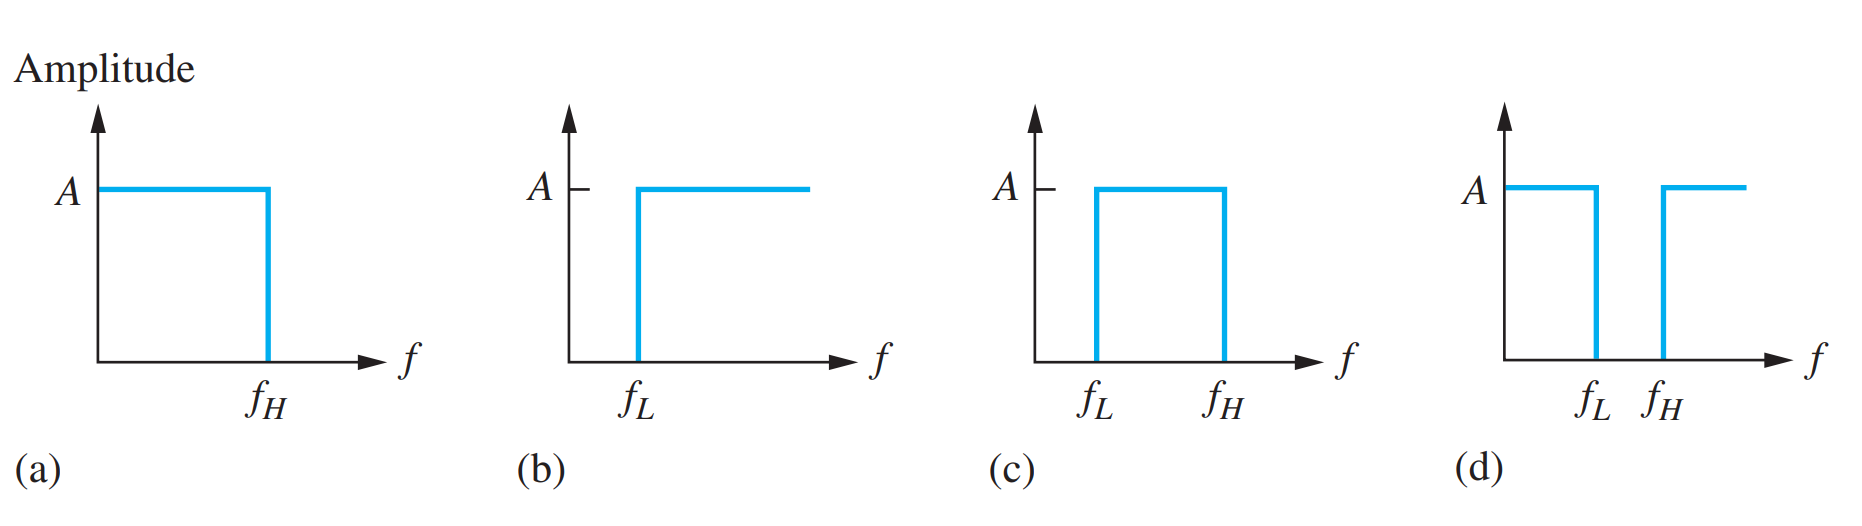
\includegraphics[keepaspectratio]{images/ImageIntroduction/TypesFilter.png}}

}

\caption{\label{fig-types}Ideal amplifier frequency responses: (a)
low-pass, (b) high-pass, (c) band-pass, (d) band-reject characteristics}

\end{figure}%

\begin{center}\rule{0.5\linewidth}{0.5pt}\end{center}

\subsection{Design Considerations}\label{design-considerations}

When designing practical filters, several key parameters must be
carefully selected to meet the desired frequency response and
performance requirements as per Baker (2010) . The following aspects are
critical in the design of active filters:

\subsubsection{\texorpdfstring{Cut-off Frequency
(\(f_0\))}{Cut-off Frequency (f\_0)}}\label{cut-off-frequency-f_0}

\begin{itemize}
\tightlist
\item
  The cutoff frequency defines the boundary between the passband and the
  stopband.
\item
  It is the frequency at which the filter's gain falls by 3 dB from its
  passband level.
\item
  For low-pass filters, frequencies below the cutoff pass with minimal
  attenuation; for high-pass filters, frequencies above the cutoff are
  passed.
\item
  Band-pass and band-stop filters have both lower and upper cutoff
  frequencies (\(f_L\) and \(f_H\)) defining their bandwidth.
\end{itemize}

\begin{figure}

\centering{

\pandocbounded{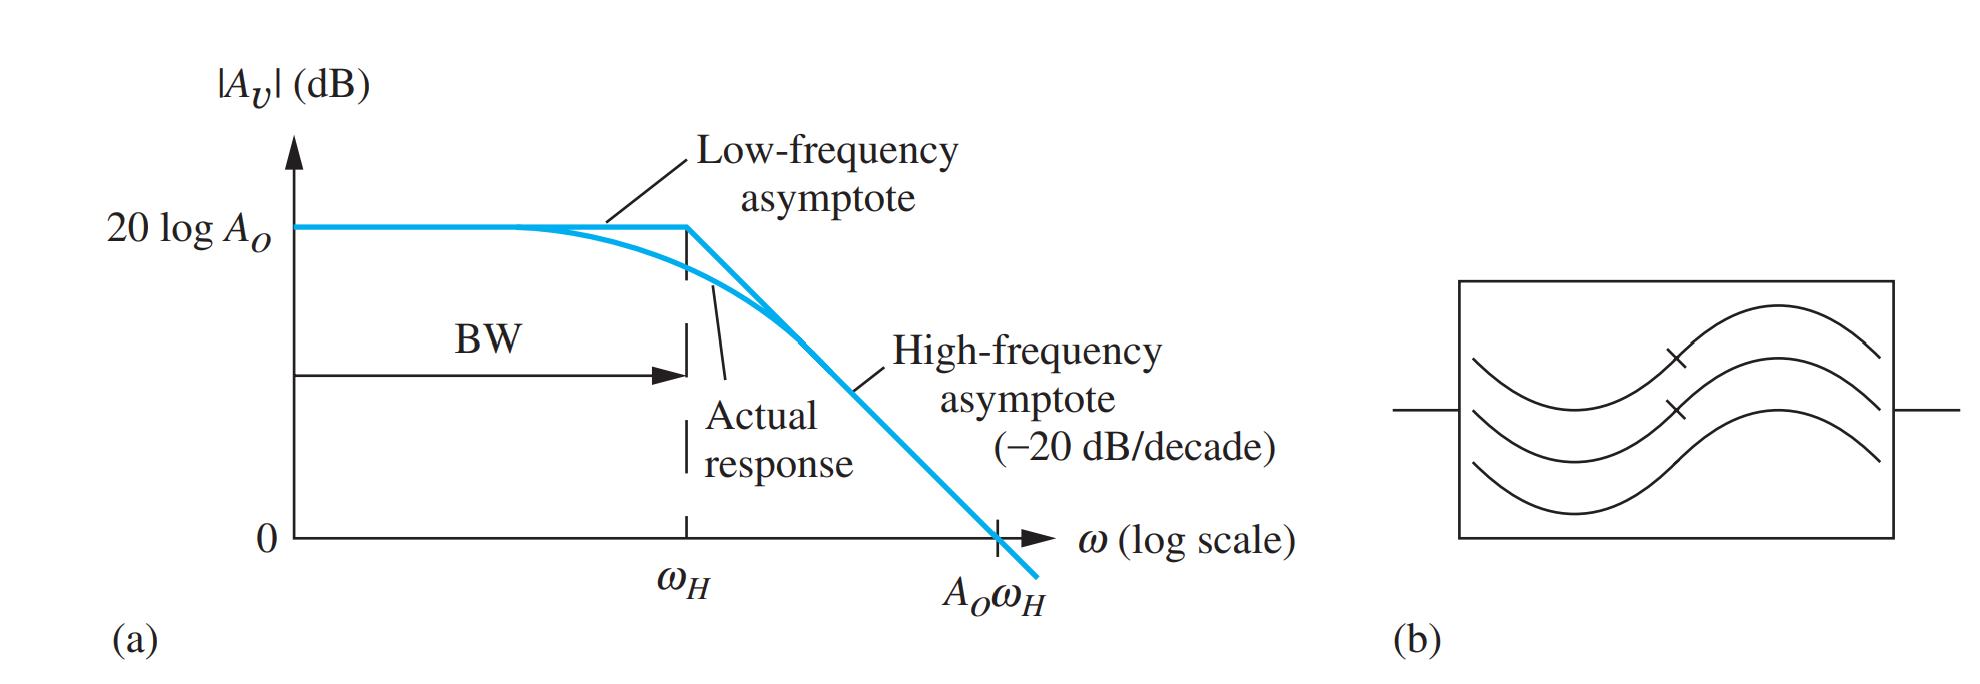
\includegraphics[keepaspectratio]{images/ImageIntroduction/lowpassF.png}}

}

\caption{\label{fig-lowpass}(a) Low-pass amplifier: BW = ωH and GBW =
AoωH ; (b) low-pass filter symbol.}

\end{figure}%

\begin{figure}

\centering{

\pandocbounded{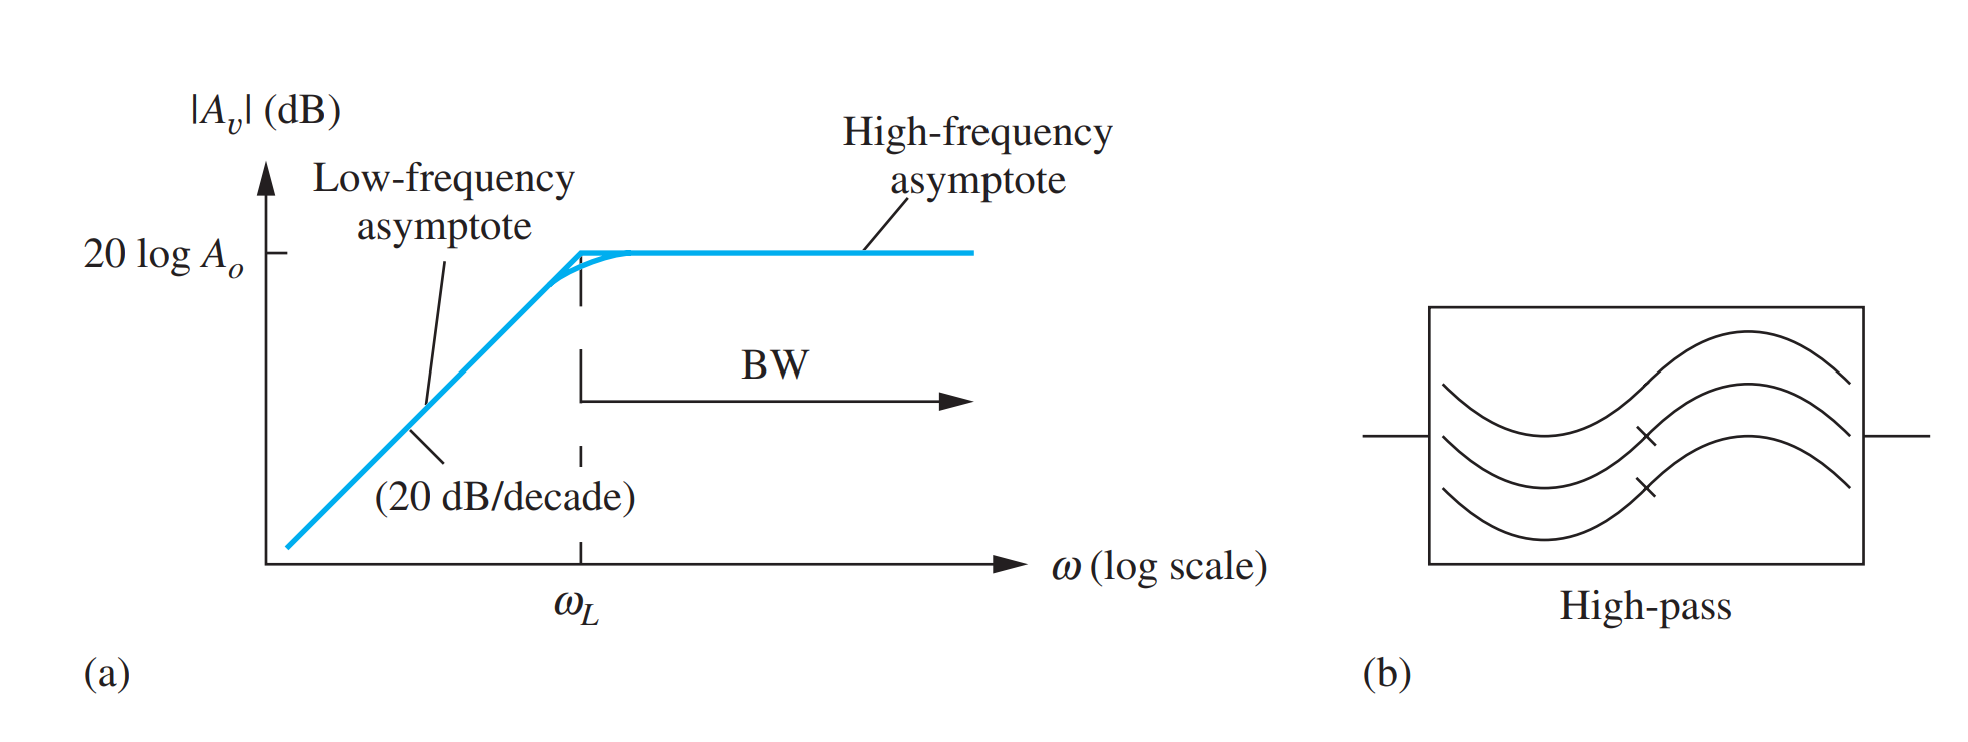
\includegraphics[keepaspectratio]{images/ImageIntroduction/highpassf.png}}

}

\caption{\label{fig-highpass}(a) High-pass amplifier; (b) high-pass
filter symbol.}

\end{figure}%

\begin{figure}

\centering{

\pandocbounded{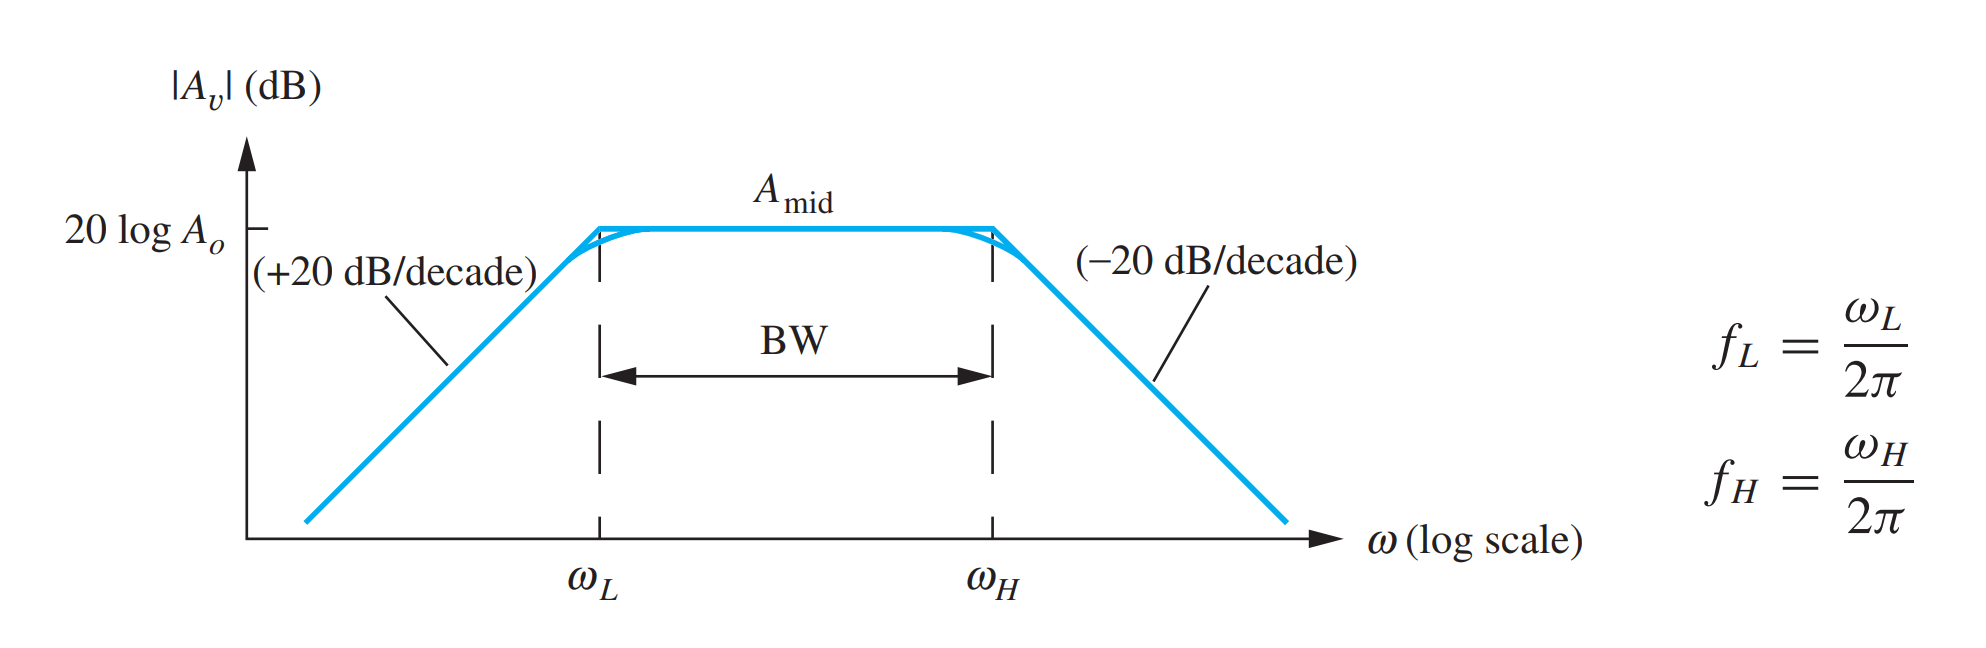
\includegraphics[keepaspectratio]{images/ImageIntroduction/bandpassF.png}}

}

\caption{\label{fig-bandpass}Band-pass amplifier.}

\end{figure}%

\begin{center}\rule{0.5\linewidth}{0.5pt}\end{center}

\subsubsection{Quality Factor (Q)}\label{quality-factor-q}

\begin{itemize}
\item
  The quality factor, Q, defines how selective the filter is around its
  center frequency.
\item
  A high Q results in a narrow, sharp response, while a low Q produces a
  broader passband.
\item
  For band-pass and band-stop filters, Q is defined as:

  \[
  Q = \frac{f_0}{f_H - f_L}
  \]
\item
  High-Q designs require precise components and stable operational
  amplifiers to avoid excessive peaking or instability.
\end{itemize}

\begin{figure}

\centering{

\pandocbounded{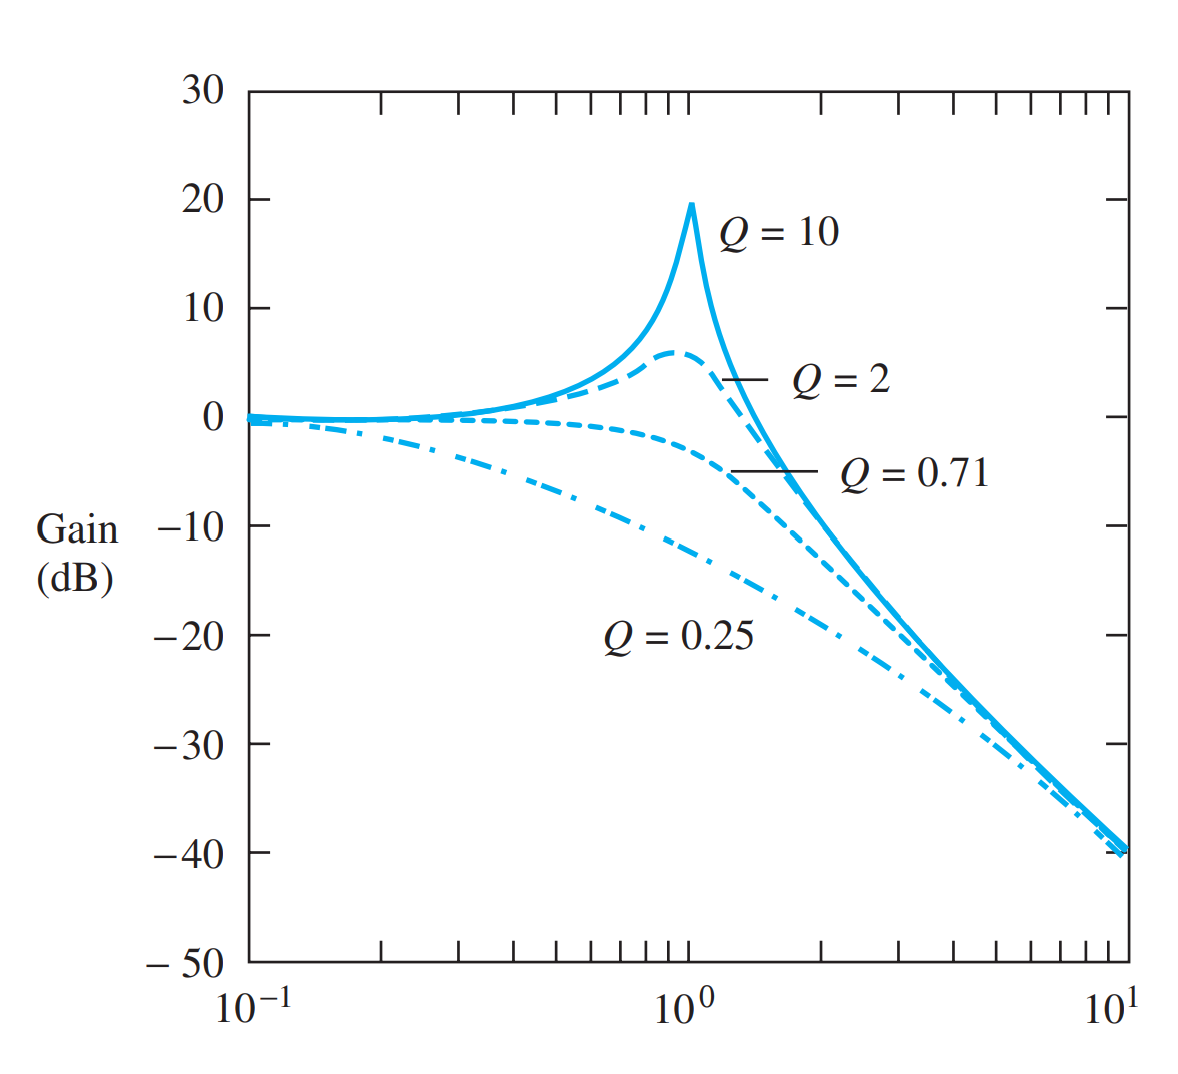
\includegraphics[keepaspectratio]{images/ImageIntroduction/lowpassQ.png}}

}

\caption{\label{fig-lowpassq}Low-pass filter response for ωo = 1 and
four values of Q.}

\end{figure}%

\begin{figure}

\centering{

\pandocbounded{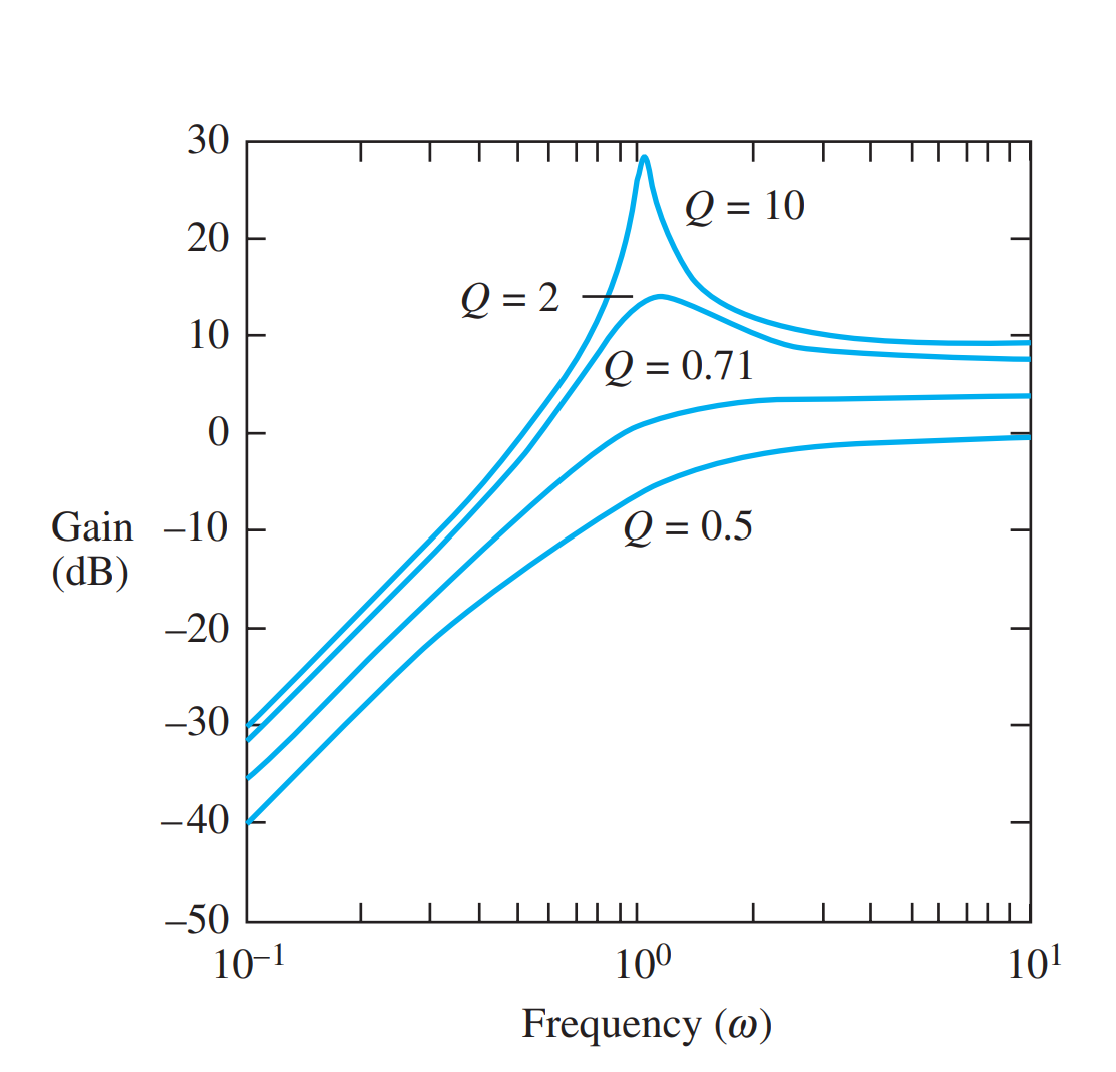
\includegraphics[keepaspectratio]{images/ImageIntroduction/highpassQ.png}}

}

\caption{\label{fig-highpassq}High-pass filter response for ωo = 1 and
four values of Q.}

\end{figure}%

\begin{figure}

\centering{

\pandocbounded{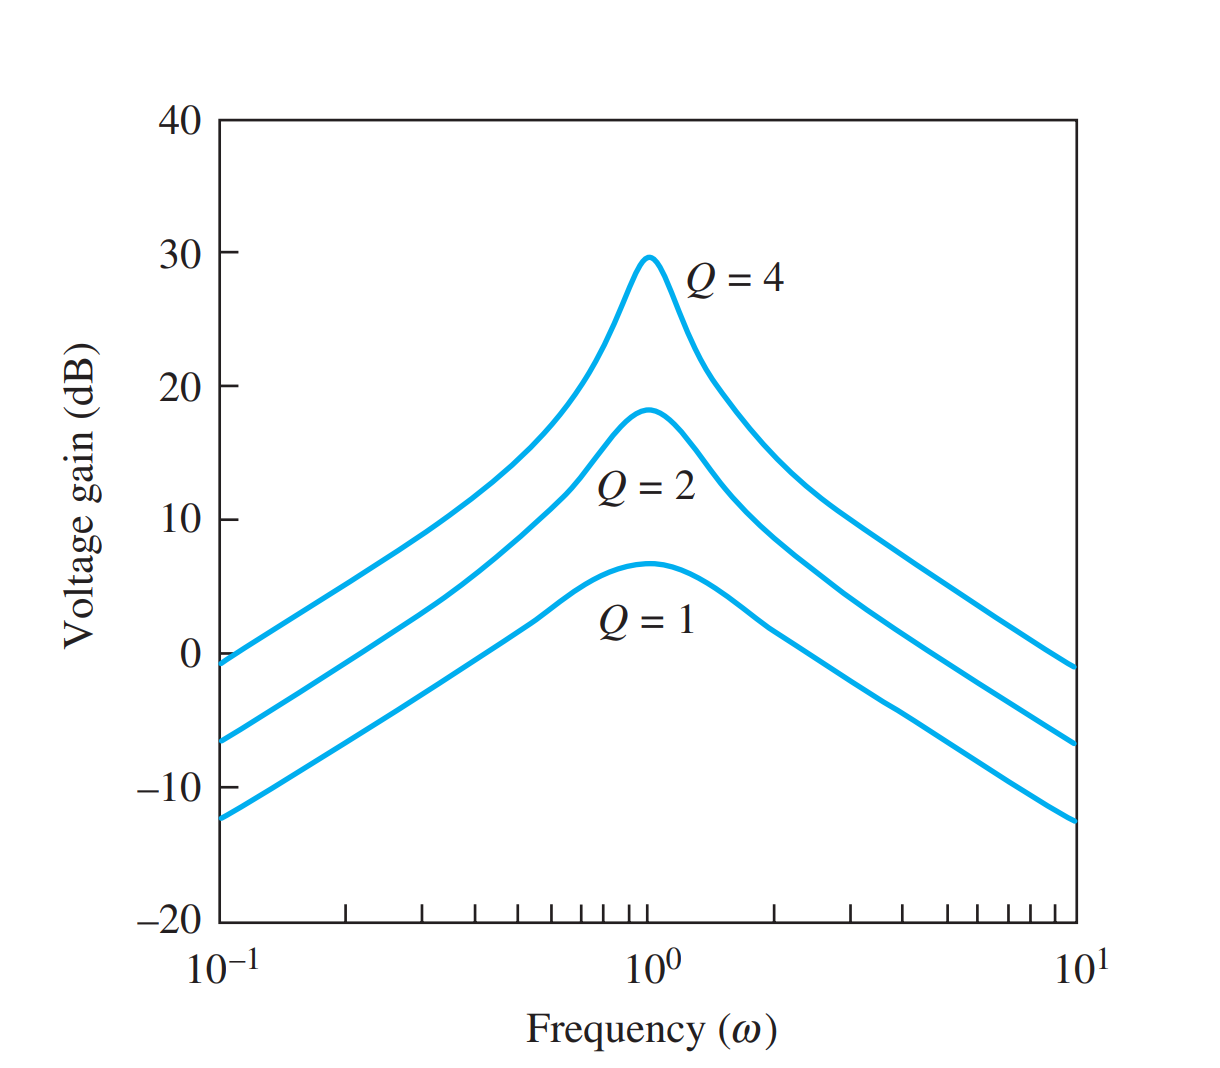
\includegraphics[keepaspectratio]{images/ImageIntroduction/bandpassQ.png}}

}

\caption{\label{fig-bandpassq}Band-pass filter response for ωo = 1 and
three values of Q assuming \(C1 = C2\) with \(R3\) = ∞}

\end{figure}%

\subsubsection{\texorpdfstring{Gain
(\(A_0\))}{Gain (A\_0)}}\label{gain-a_0}

\begin{itemize}
\item
  The gain, \(A_0\), sets the amplitude level in the filter's passband
  (midband).
\item
  Expressed either as a linear ratio or in decibels (dB):

  \[
  A_0 \;(\text{dB}) = 20 \log_{10}(A_0)
  \]
\item
  In active filter circuits, \(A_0\) is determined by resistor ratios
  and must be chosen to provide adequate signal strength without causing
  distortion.
\end{itemize}

\subsubsection{Natural Frequency
(ω₀)}\label{natural-frequency-ux3c9ux2080}

\begin{itemize}
\item
  The natural frequency, denoted ω₀, determines the center frequency of
  resonance in band-pass and band-stop filters and corresponds to the
  cutoff frequency in low-pass and high-pass filters.
\item
  It is given by:

  \[
  \omega_0 = 2\pi f_0
  \]
\item
  Selecting ω₀ correctly ensures the filter passes or attenuates the
  intended frequency range.
\end{itemize}

\subsubsection{Filter Order}\label{filter-order}

\begin{itemize}
\tightlist
\item
  The filter order represents the number of reactive components
  (capacitors or inductors) influencing the frequency response.
\item
  Higher-order filters provide steeper roll-off slopes and better
  attenuation of unwanted frequencies.
\item
  Each order increases the slope by approximately −20 dB per decade:

  \begin{itemize}
  \tightlist
  \item
    1st-order → −20 dB/decade
  \item
    2nd-order → −40 dB/decade
  \end{itemize}
\end{itemize}

\begin{center}\rule{0.5\linewidth}{0.5pt}\end{center}

\subsection{Practical Design
Implications}\label{practical-design-implications}

\begin{itemize}
\tightlist
\item
  The choice of Q and ω₀ determines whether the filter achieves the
  desired bandwidth and selectivity.
\item
  Higher Q increases sensitivity to component tolerances and can
  introduce peaking or ringing in the time domain.
\item
  Operational amplifiers used in active filters must offer sufficient
  bandwidth and low noise to maintain signal integrity.
\item
  Gain settings must balance signal amplitude requirements with
  stability and noise performance.
\end{itemize}

These considerations are essential to ensure that real filters not only
match theoretical frequency responses but also operate reliably and
efficiently in practical applications.

\begin{center}\rule{0.5\linewidth}{0.5pt}\end{center}

\chapter{Operational Amplifiers}\label{operational-amplifiers}

Operational amplifiers (op amps) are fundamental building blocks in
analog circuit design, widely used for amplification, filtering, signal
conditioning, and mathematical operations. Their design and layout
involve both ideal and non-ideal considerations to ensure optimal
performance in practical applications.

\section{Common Configurations}\label{common-configurations}

\subsection{Inverting Amplifier}\label{inverting-amplifier}

An inverting-amplifier circuit is built by grounding the positive input
of the operational amplifier and connecting resistors \(R_1\) and
\(R_2\), called the feedback network, between the inverting input and
the signal source and amplifier output node, respectively, as in
Figure~\ref{fig-inverter}.

\begin{figure}

\centering{

\pandocbounded{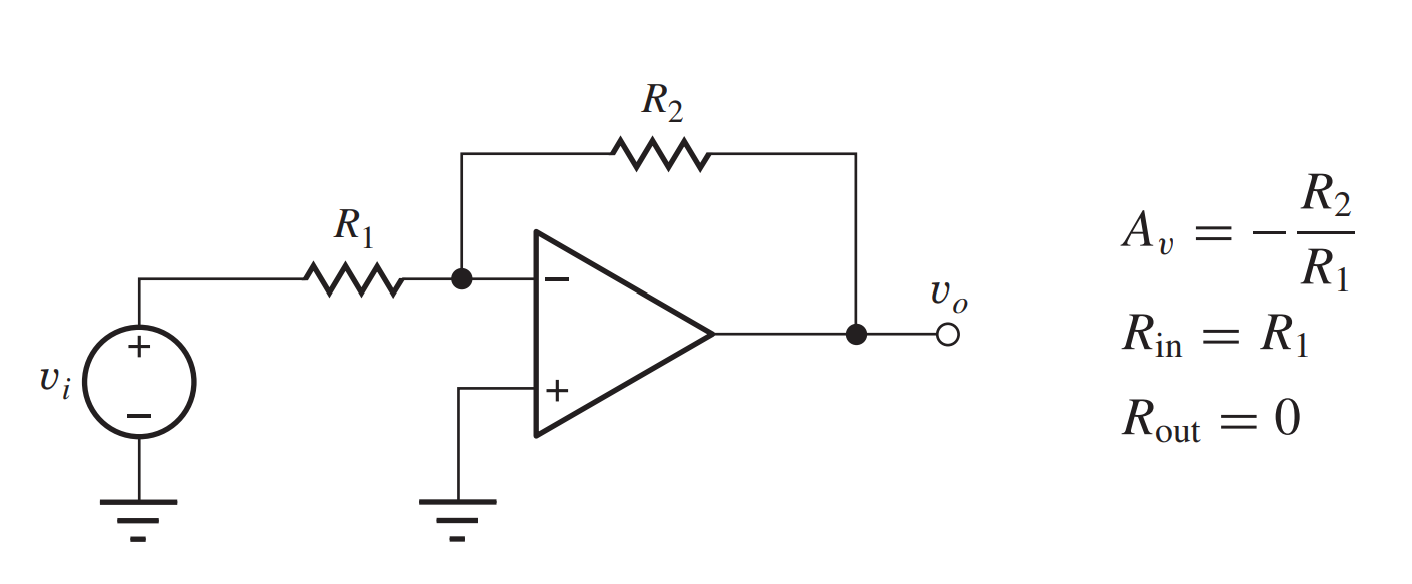
\includegraphics[keepaspectratio]{images/ImageIntroduction/Inverting.png}}

}

\caption{\label{fig-inverter}Inverting Amplifier.}

\end{figure}%

\begin{center}\rule{0.5\linewidth}{0.5pt}\end{center}

\subsection{Summing Amplifier}\label{summing-amplifier}

Operational amplifiers can also be used to combine signals using the
summing-amplifier circuit depicted in Fig. 10.24. Here, two input
sources \(v_1\) and \(v_2\) are connected to the inverting input of the
amplifier through resistors \(R_1\) and \(R_2\). Because the negative
amplifier input represents a virtual ground,

\(i_1 = \frac{v_1}{R_1}\) , \(i_2 = \frac{v_2}{R_2}\) ,
\(i_3 = -\frac{v_o}{R_3}\)

Since the input current into the op amp (\(i^{-}\)) is effectively zero,
the currents satisfy: \(i_3 = i_1 + i_2\).

\[
v_o = -\left(\frac{R_3}{R_1} v_1 \;+\; \frac{R_3}{R_2} v_2\right)
\]

The output voltage sums the scaled replicas of the two input voltages,
and the scale factors for the two inputs may be independently adjusted
through the choice of resistors \(R_1\) and \(R_2\). These two inputs
can be scaled independently because of the virtual ground maintained at
the inverting-input terminal of the op amp. The inverting-amplifier
input node is also commonly called the summing junction because currents
\(i_1\) and \(i_2\) are ``summed'' at this node and forced through the
feedback resistor \(R_3\). Although the amplifier in
Figure~\ref{fig-adder} has only two inputs, any number of inputs can be
connected to the summing junction through additional resistors.

\begin{figure}

\centering{

\pandocbounded{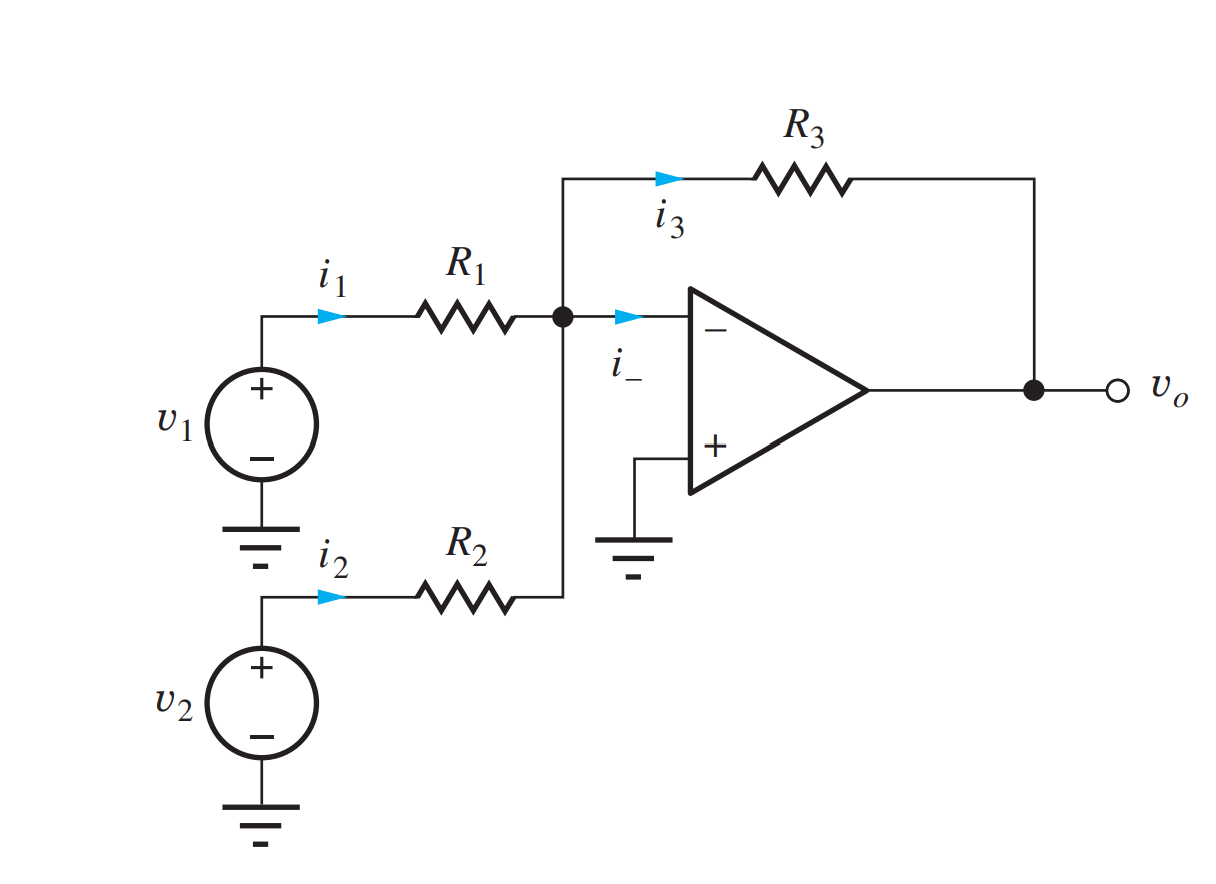
\includegraphics[keepaspectratio]{images/ImageIntroduction/Adder.png}}

}

\caption{\label{fig-adder}Summing Amplifier.}

\end{figure}%

\begin{center}\rule{0.5\linewidth}{0.5pt}\end{center}

\subsection{Integrator}\label{integrator}

The \textbf{integrator} is another important building block that uses an
operational amplifier with frequency-dependent feedback. In the
integrator circuit, the feedback resistor \(R_2\) of a standard
inverting amplifier is replaced by a capacitor \(C\), as shown in
Figure~\ref{fig-inte}. This configuration enables the circuit to perform
integration of the input signal and provides a valuable example for op
amp circuit analysis in the time domain.

Because the inverting input of the op amp behaves as a virtual ground,
the input current and the capacitor current can be written as:
\(i_i = \frac{v_i}{R}\), \(i_c = -C \frac{d v_o}{dt}\)

\begin{figure}

\centering{

\pandocbounded{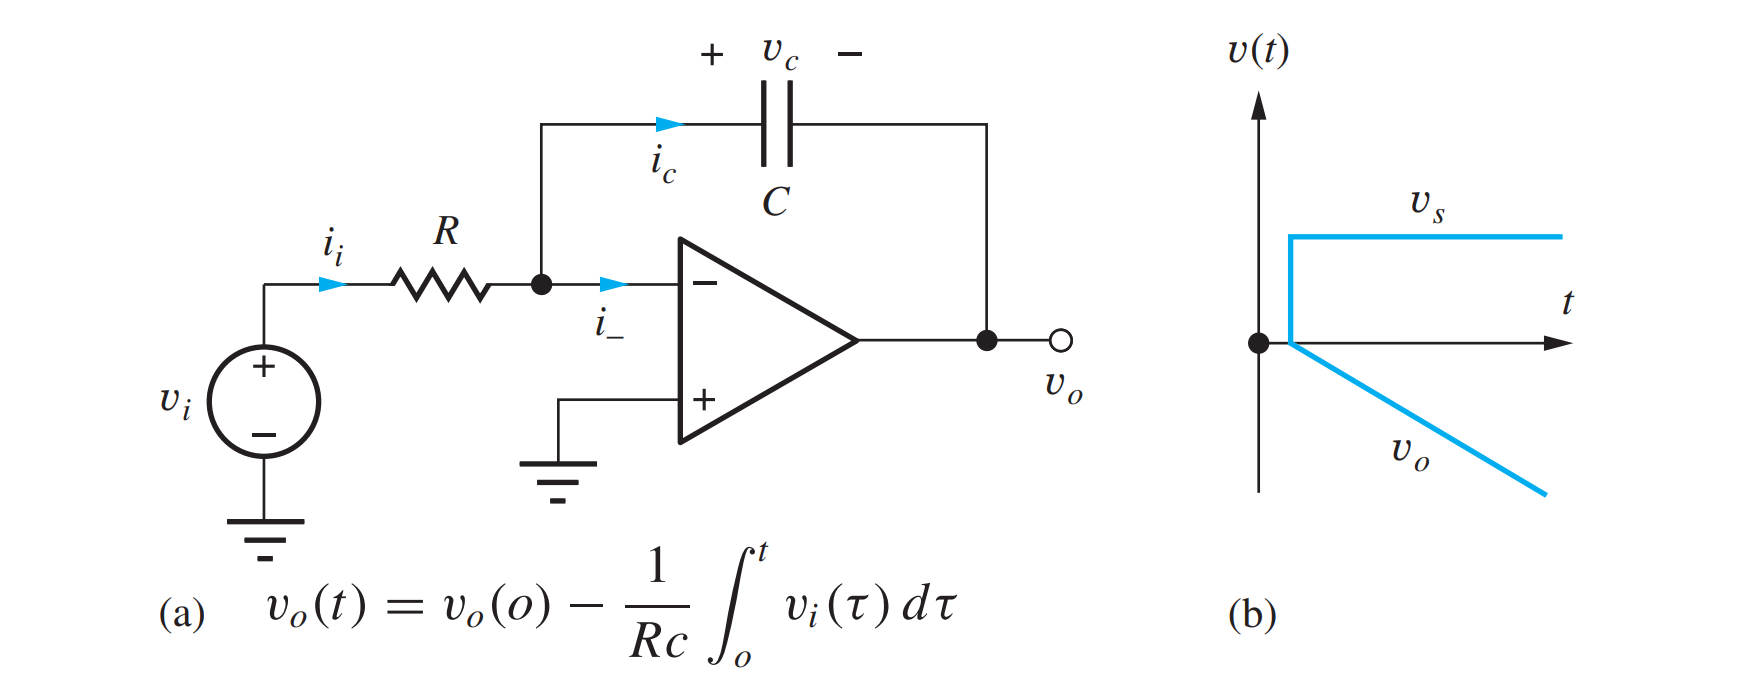
\includegraphics[keepaspectratio]{images/ImageIntroduction/Integrator.png}}

}

\caption{\label{fig-inte}(a) The integrator circuit; (b) output voltage
for a step-function input with \(v_C\) (0) = 0.}

\end{figure}%

For an ideal op amp, the input current into the inverting terminal,
\(i^-\), is zero. Thus \(i_c = i_i\)

Equating the two expressions and integrating both sides gives:

\[
d v_o = -\frac{1}{RC} \, v_i \, d\tau
\]

which integrates to:

\[
v_o(t) = v_o(0) - \frac{1}{RC} \int_0^t v_i(\tau) \, d\tau
\]

where \(v_o(0)\) represents the initial voltage at the op amp output,
determined by the initial voltage across the capacitor at \(t=0\):

\[
v_o(0) = -v_C(0)
\]

Therefore, the voltage at the output of the integrator at any time \(t\)
equals the initial capacitor voltage minus the integral of the input
signal from the starting time \(t=0\).

\subsubsection{Understanding Integrator Circuit
Operation}\label{understanding-integrator-circuit-operation}

The virtual ground at the inverting input of the op amp causes input
voltage vi to appear directly across resistor R establishing an input
current \(v_i/R\). As the input current flows out through \(C\), the
capacitor accumulates a charge equal to the integral of the current,
\(Q_C = \frac{1}{C} \int i \, dt\) , and the overall scale factor
becomes \(-\frac{1}{RC}\) Baker (2010).

\chapter{General KHN Biquad Filters}\label{general-khn-biquad-filters}

The KHN biquad is an active filter topology that uses three operational
amplifiers (op-amps) to implement a second-order filter. It is called a
``biquad'' because it realizes a biquadratic transfer function, which is
a ratio of two quadratic polynomials. The KHN configuration is notable
for providing simultaneous access to low-pass, high-pass, and bandpass
outputs from a single circuit, making it highly versatile. The KHN
filter is based on a state-variable filter approach, where the circuit
maintains internal state variables (typically voltages) that represent
the system's dynamics. This allows for independent control of the
filter's key parameters: the natural frequency (\(w_0\)), quality factor
(\(Q\)), and gain (\(H\)) {``EE315 Course''} (2025).

\section{Circuit Configuration}\label{circuit-configuration}

The KHN biquad filter consists of three main op-amp stages:

\begin{itemize}
\tightlist
\item
  Two Integrators: These form the core of the state-variable filter,
  creating a feedback loop that defines the second-order dynamics.
\item
  A Summing Amplifier: This combines the input signal and feedback
  signals to produce the desired filter outputs.
\end{itemize}

\textbf{Circuit Structure}

First Integrator: Integrates the input signal or a combination of the
input and feedback signals. Second Integrator: Integrates the output of
the first integrator, producing the low-pass output. Summing Amplifier:
Combines signals to produce the high-pass and bandpass outputs.

The circuit typically includes resistors and capacitors to set the
filter parameters, with the op-amps operating in a linear mode. A
simplified block diagram of the KHN biquad is as follows:

Input → Summing Amplifier → First Integrator → Second Integrator →
Low-Pass Output Feedback loops from the integrators feed back to the
summing amplifier. The high-pass output is taken from the summing
amplifier, the bandpass from the first integrator, and the low-pass from
the second integrator.

\begin{figure}

\centering{

\pandocbounded{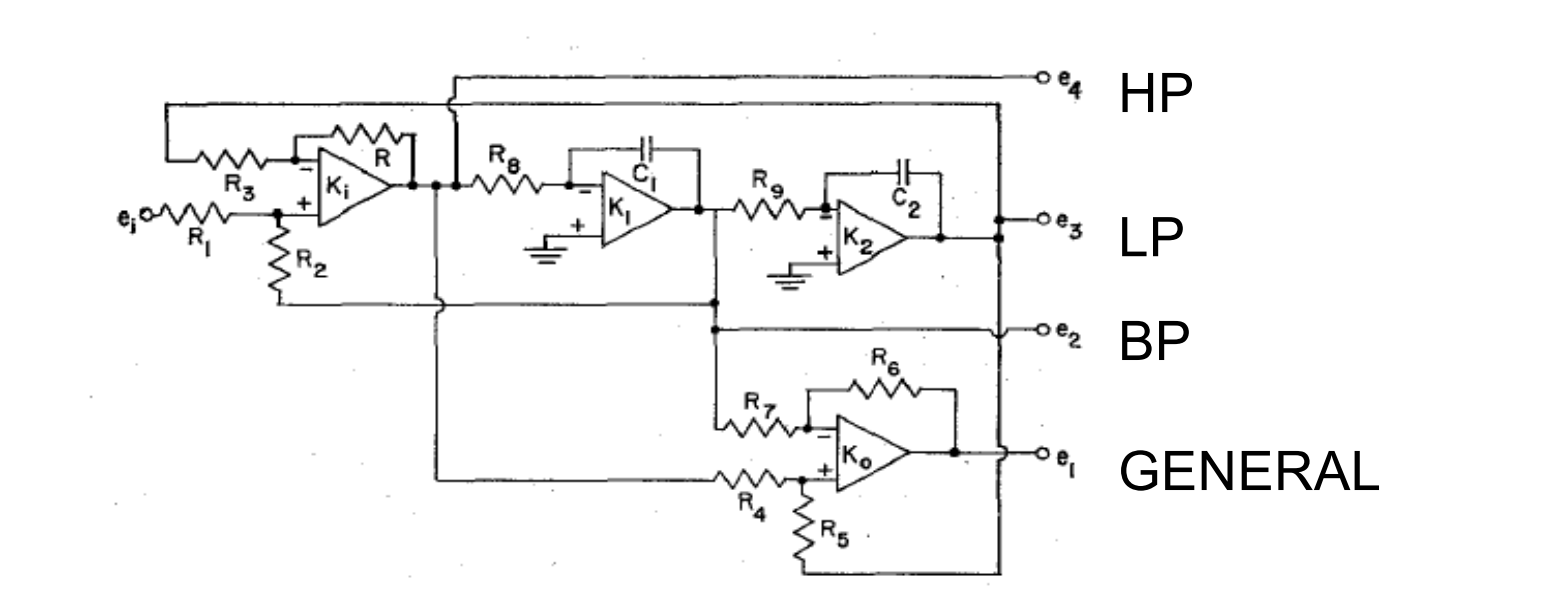
\includegraphics[keepaspectratio]{images/ImageIntroduction/KhnBiquad.png}}

}

\caption{\label{fig-khn}Block diagram of the KHN biquad.}

\end{figure}%

A typical KHN biquad circuit includes:

Resistors (R₁, R₂, etc.) to control gain and feedback. Capacitors (C₁,
C₂) to set the frequency response. Three op-amps configured as
integrators and a summer.

\section{Transfer Functions}\label{transfer-functions}

The KHN biquad provides three standard outputs: high-pass, bandpass, and
low-pass. The transfer functions for these outputs are derived from the
circuit's feedback structure and can be expressed in the s-domain
(Laplace domain) as follows, assuming ideal op-amps: General Biquadratic
Transfer Function The general form of a second-order filter transfer
function is:
\[T(s) = \frac{N(s)}{D(s)} = \frac{a_2 s^2 + a_1 s + a_0}{s^2 + \frac{\omega_0}{Q} s + \omega_0^2}\]
Where:

( \(s\) ) is the complex frequency variable. ( \(\omega_0\)) is the
natural angular frequency (related to the cutoff or center frequency). (
\(Q\) ) is the quality factor, which determines the sharpness of the
resonance. ( \(a_2\), \(a_1\), \(a_0\) ) determine the filter type
(high-pass, bandpass, low-pass, etc.).

For the KHN biquad, the specific transfer functions for each output are:

Low-Pass Output:

\[H_{LP}(s) = \frac{\omega_0^2}{s^2 + \frac{\omega_0}{Q} s + \omega_0^2}\]

This passes low frequencies and attenuates high frequencies.

Bandpass Output:

\[H_{BP}(s) = \frac{\frac{\omega_0}{Q} s}{s^2 + \frac{\omega_0}{Q} s + \omega_0^2}\]

This passes a band of frequencies centered around ( \$\omega\_0 \$).

High-Pass Output:

\[H_{HP}(s) = \frac{s^2}{s^2 + \frac{\omega_0}{Q} s + \omega_0^2}\]

This passes high frequencies and attenuates low frequencies.

By adjusting resistor and capacitor values, other filter types (e.g.,
notch or all-pass) can be derived by combining these outputs with
appropriate gain and summation. Key Parameters

Natural Frequency (( \(\omega_0\) )): Determines the cutoff or center
frequency of the filter. For a KHN biquad, it is typically set by the
resistors and capacitors in the integrator stages:

\[\omega_0 = \frac{1}{\sqrt{R_1 R_2 C_1 C_2}}\]

Quality Factor (Q): Controls the bandwidth and resonance of the filter.
It is set by the feedback resistors:

\[Q = \frac{\sqrt{R_1 R_2 C_1 C_2}}{R_f (C_1 + C_2)}\] where ( \(R_f\) )
is the feedback resistor in the summing stage.

Gain (H): The gain of each output (low-pass, bandpass, high-pass) can be
adjusted by scaling the resistors in the summing amplifier.

\section{Design Parameters and
Tuning}\label{design-parameters-and-tuning}

The KHN biquad is highly flexible because its key parameters ((
\(\omega_0\) ), ( \(Q\) ), and gain) can be tuned independently:

Tuning ( \(\omega_0\) ): Adjust the resistors (( \(R_1\), \(R_2\) )) or
capacitors (( \(C_1\), \(C_2\) )) in the integrator stages. Changing
these values affects the frequency without altering ( \(Q\) ) or gain
significantly.

Tuning ( \(Q\) ): Adjust the feedback resistor (( \(R_f\) )) in the
summing stage. A smaller ( \(R_f\) ) increases ( \(Q\) ), making the
filter more selective (narrower bandwidth).

Tuning Gain: Adjust the resistors in the summing amplifier to scale the
output amplitude for each filter type.

This independent control is a significant advantage over other biquad
topologies, such as the Sallen-Key filter, where parameters are often
interdependent.

\chapter{Filter Design}\label{filter-design}

\section{Objective}\label{objective}

The objective is to design a biquadratic filter with the \textbf{corner
frequency = 1000Hz and Q = 10.}

\section{Behavioural Model}\label{behavioural-model}

This is a theoretical model so as to understand the acheivable taget
using the transfer functions of active filters such as low pass, high
pass, band pass and band stop filter. The basics is refered from Baker
(2010).

\subsection{Behavioural model of active filters using
Python}\label{behavioural-model-of-active-filters-using-python}

Low Pass Filter :

\[
H(s) = \frac{H_0}{(1+\frac{s}{w_0 Q}+\frac{s^2}{w_0^2})} = \frac{1}{1e-06s^2 + 0.0001s + 1}
\]

High Pass Filter:

\[H(s) = \frac{V_{01}}{V_i} = \frac{H_0\frac{s^2}{w_0^2}}{(1+\frac{s}{w_0 Q}+\frac{s^2}{w_0^2})} = \frac{1e-06 s^2}{1e-06s^2 + 0.0001s + 1}\]

Band Pass Filter:

\[H(s) = \frac{V_{02}}{V_i} = \frac{-H_0\frac{s}{w_0}}{(1+\frac{s}{w_0 Q}+\frac{s^2}{w_0^2})} = \frac{-0.001 s}{1e-06s^2 + 0.0001s + 1}\]

Band Stop Filter:

\[H(s) = \frac{V_{04}}{V_i} = \frac{(1 + \frac{s^2}{w_0^2})H_0}{(1+\frac{s}{w_0 Q}+\frac{s^2}{w_0^2})} = \frac{( 1 + 1e-06 s^2 ) 1}{1e-06s^2 + 0.0001s + 1}\]

where, \(Q\)= Quality Factor, \(H_0\)= Gain, \(\omega_0\)=Corner
Frequency

The python code for generating frequency response and step response is
given
\href{https://github.com/oreymaonr/hsb-amcd-sose2025-5/blob/main/content/plotfn.py}{here.}

\subsubsection{Behavioural phase and magnitude plots (Frequency response
plots)}\label{behavioural-phase-and-magnitude-plots-frequency-response-plots}

These plots as per Figure~\ref{fig-behavioural-frequency} are generated
by the transfer function equations using \texttt{signal.bode()} of
python scipy module.

\begin{figure}

\begin{minipage}{0.50\linewidth}

\centering{

\pandocbounded{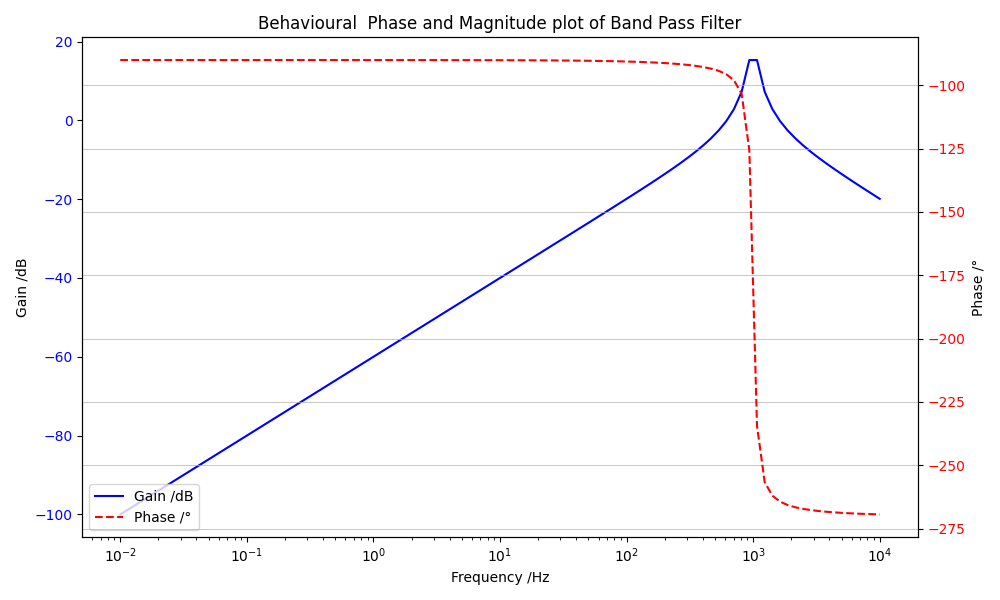
\includegraphics[keepaspectratio]{images/behaviourial/bode/bpf.png}}

}

\subcaption{\label{fig-bpf}Band Pass}

\end{minipage}%
%
\begin{minipage}{0.50\linewidth}

\centering{

\pandocbounded{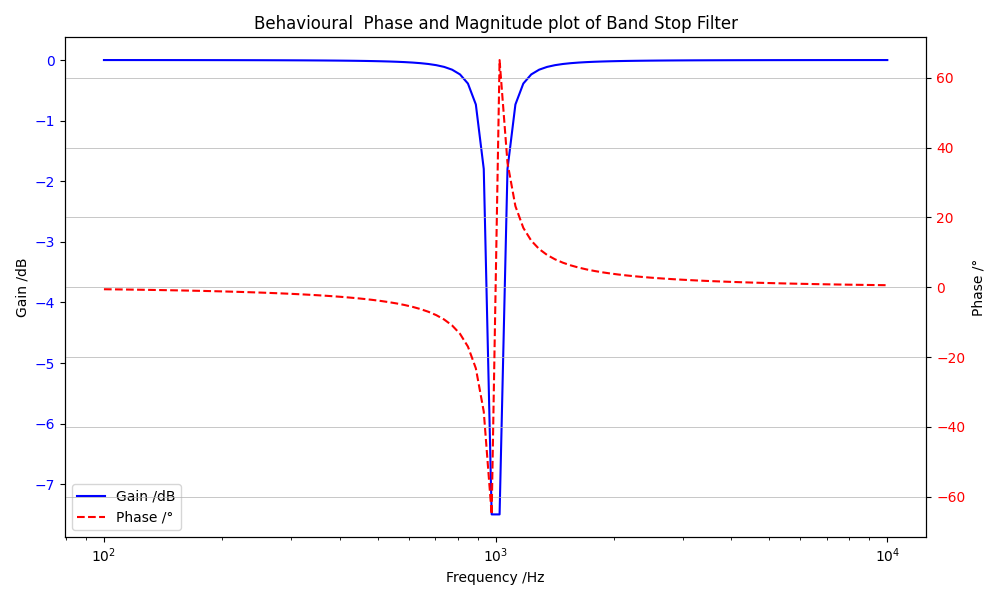
\includegraphics[keepaspectratio]{images/behaviourial/bode/bsf.png}}

}

\subcaption{\label{fig-bpf}Band Stop}

\end{minipage}%
\newline
\begin{minipage}{0.50\linewidth}

\centering{

\pandocbounded{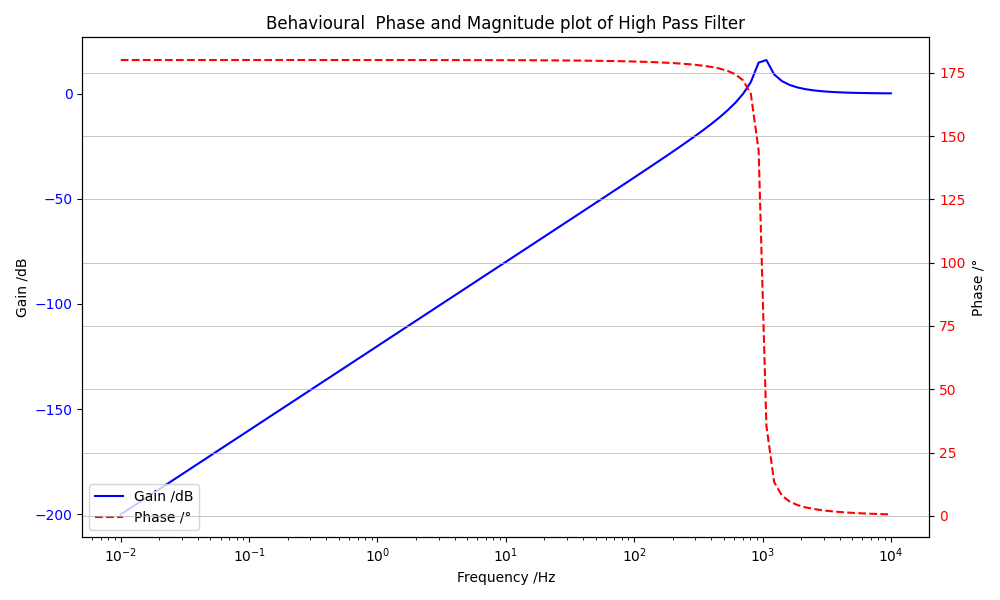
\includegraphics[keepaspectratio]{images/behaviourial/bode/hpf.png}}

}

\subcaption{\label{fig-bpf}High Pass}

\end{minipage}%
%
\begin{minipage}{0.50\linewidth}

\centering{

\pandocbounded{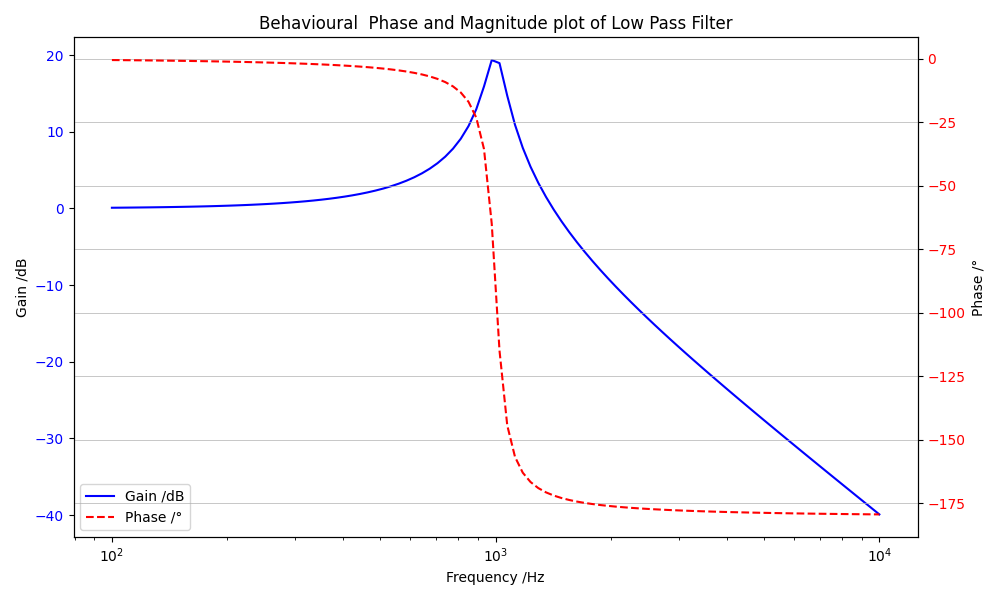
\includegraphics[keepaspectratio]{images/behaviourial/bode/lpf.png}}

}

\subcaption{\label{fig-bpf}Low Pass}

\end{minipage}%

\caption{\label{fig-behavioural-frequency}Behavioural phase and
magnitude plots}

\end{figure}%

\subsubsection{Behavioural Steady State response (Transcient response
plots)}\label{behavioural-steady-state-response-transcient-response-plots}

These plots at Figure~\ref{fig-behavioural-transcient} is generated
solely by \texttt{signal.step()} from scipy python module.

\begin{figure}

\begin{minipage}{0.50\linewidth}

\centering{

\pandocbounded{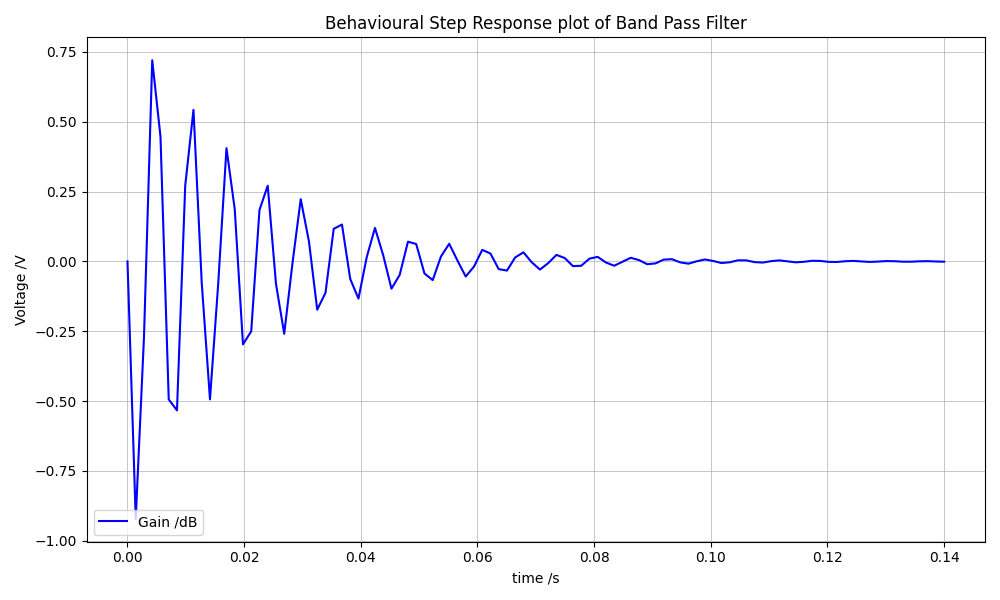
\includegraphics[keepaspectratio]{images/behaviourial/Transcient/bpf.png}}

}

\subcaption{\label{fig-bpf}Band Pass}

\end{minipage}%
%
\begin{minipage}{0.50\linewidth}

\centering{

\pandocbounded{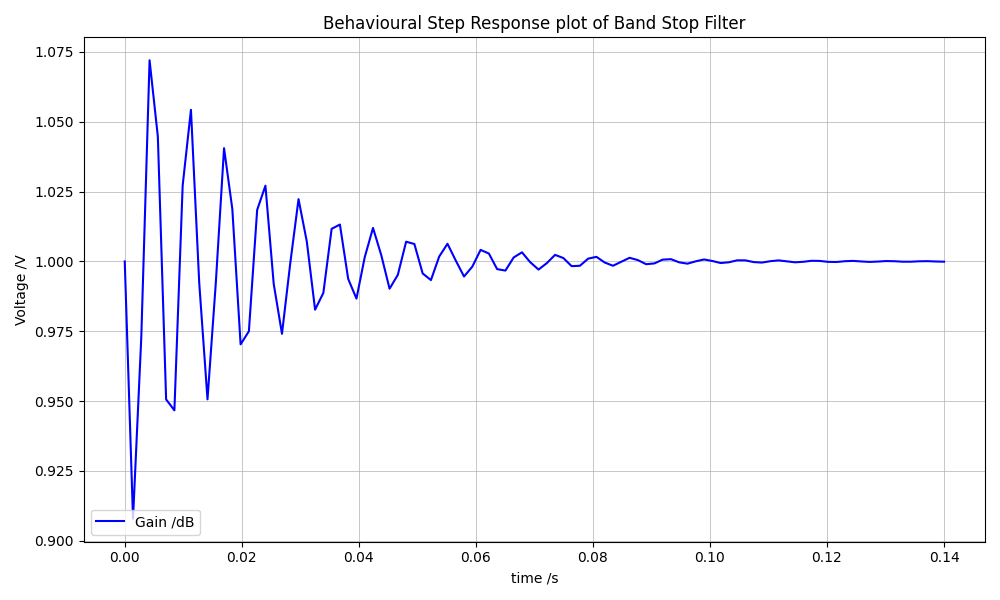
\includegraphics[keepaspectratio]{images/behaviourial/Transcient/bsf.png}}

}

\subcaption{\label{fig-bpf}Band Stop}

\end{minipage}%
\newline
\begin{minipage}{0.50\linewidth}

\centering{

\pandocbounded{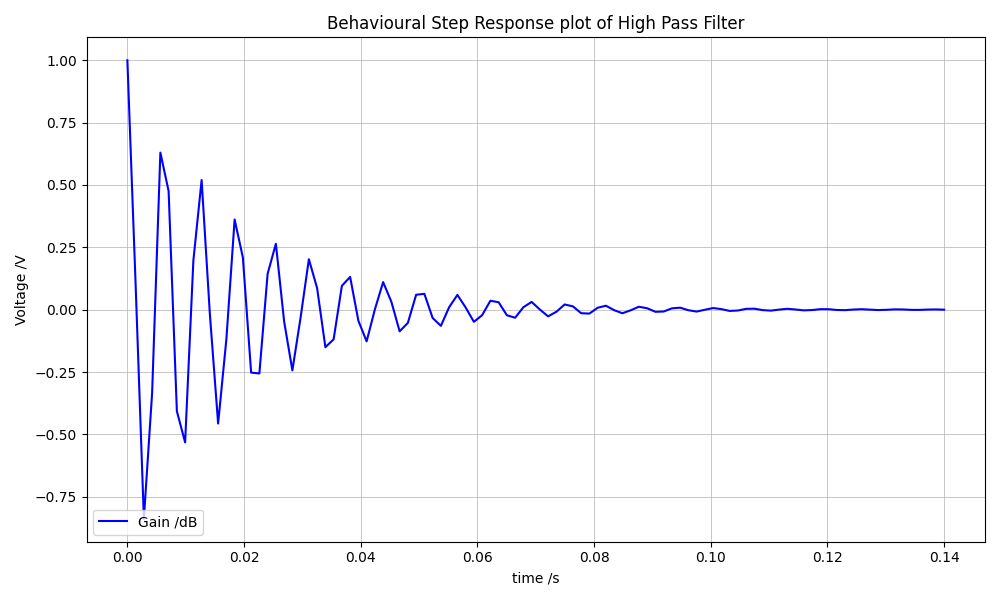
\includegraphics[keepaspectratio]{images/behaviourial/Transcient/hpf.png}}

}

\subcaption{\label{fig-bpf}High Pass}

\end{minipage}%
%
\begin{minipage}{0.50\linewidth}

\centering{

\pandocbounded{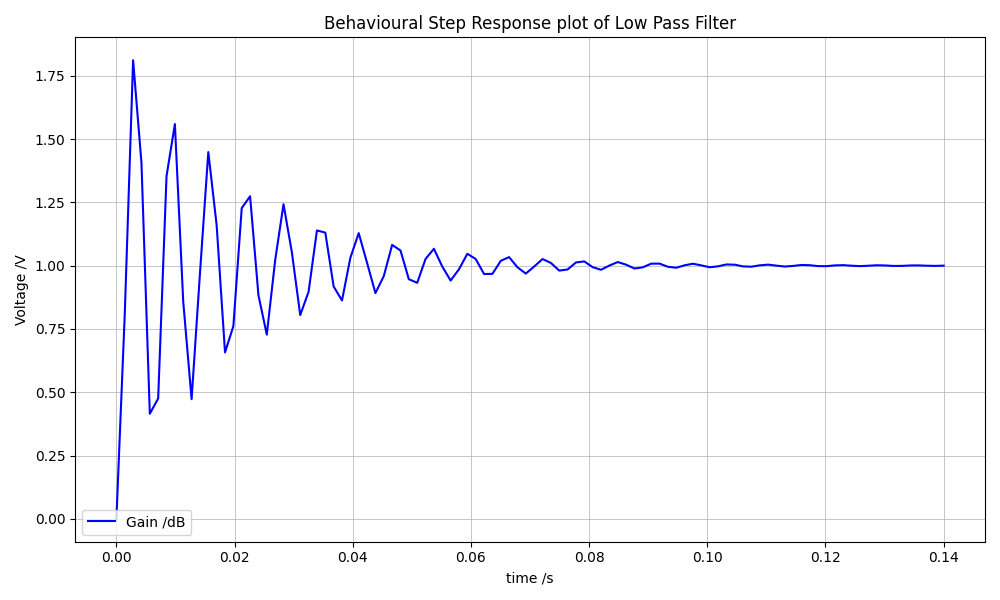
\includegraphics[keepaspectratio]{images/behaviourial/Transcient/lpf.png}}

}

\subcaption{\label{fig-bpf}Low Pass}

\end{minipage}%

\caption{\label{fig-behavioural-transcient}Behavioural phase and
magnitude plots}

\end{figure}%

\subsubsection{Behavioural pole-zero
plots}\label{behavioural-pole-zero-plots}

These plots at Figure~\ref{fig-behavioural-pole-zero} is generated by
\texttt{control.poles()} and \texttt{control.step\_info()} from control
python module.

\begin{figure}

\begin{minipage}{0.50\linewidth}

\centering{

\pandocbounded{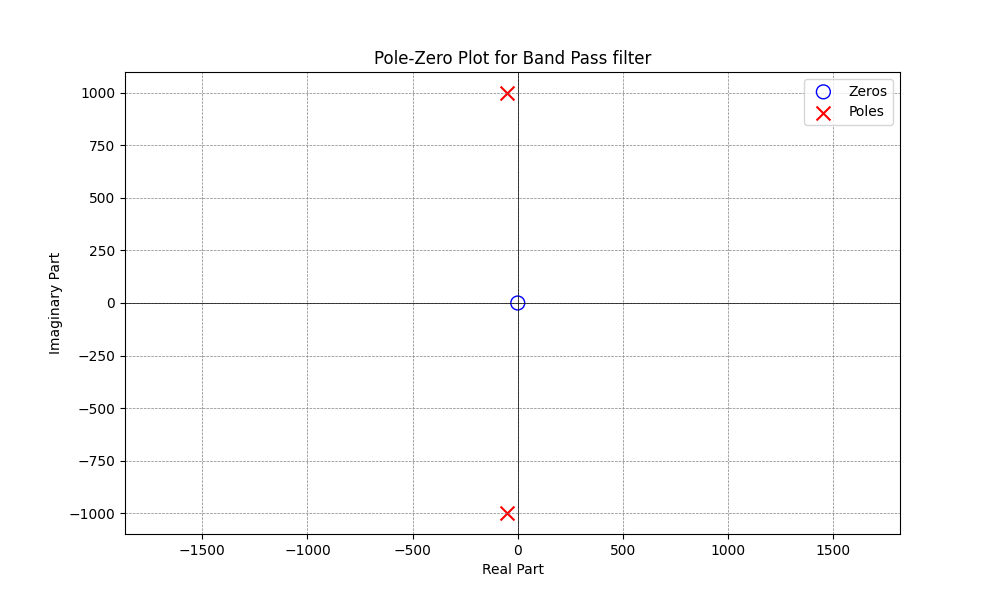
\includegraphics[keepaspectratio]{images/behaviourial/pzplot/bpf.png}}

}

\subcaption{\label{fig-bpf}Band Pass}

\end{minipage}%
%
\begin{minipage}{0.50\linewidth}

\centering{

\pandocbounded{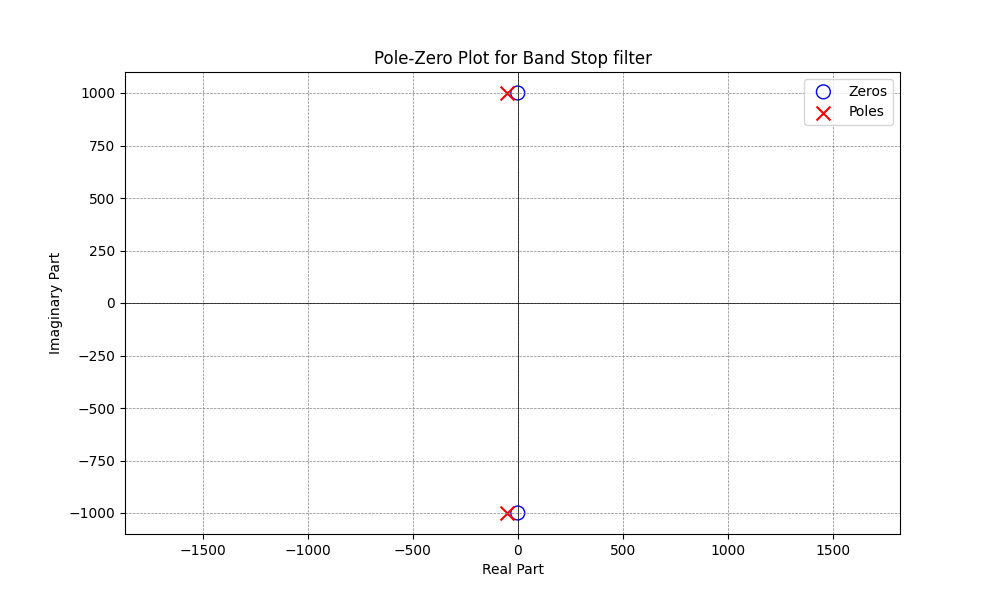
\includegraphics[keepaspectratio]{images/behaviourial/pzplot/bsf.png}}

}

\subcaption{\label{fig-bpf}Band Stop}

\end{minipage}%
\newline
\begin{minipage}{0.50\linewidth}

\centering{

\pandocbounded{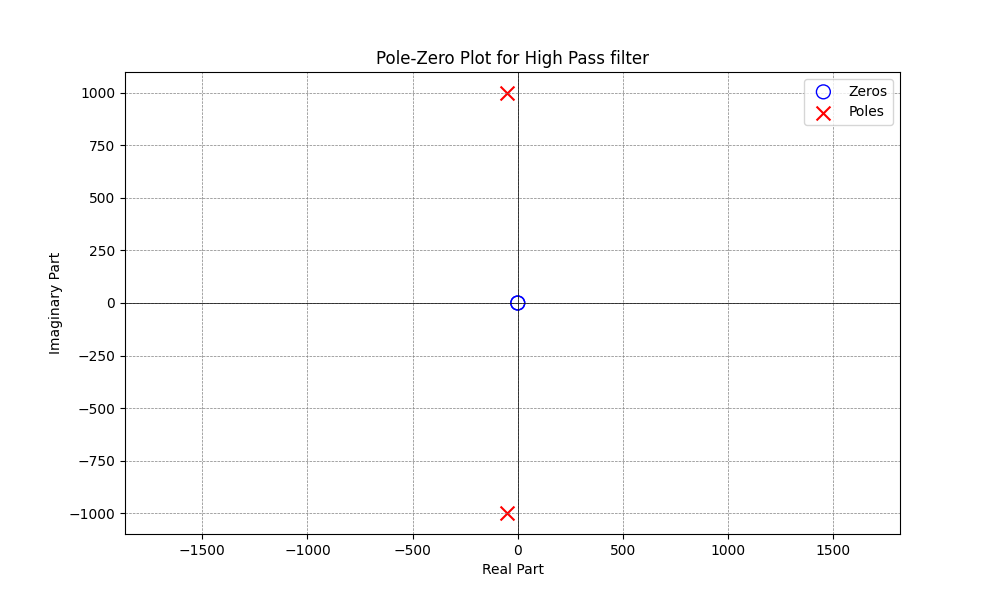
\includegraphics[keepaspectratio]{images/behaviourial/pzplot/hpf.png}}

}

\subcaption{\label{fig-bpf}High Pass}

\end{minipage}%
%
\begin{minipage}{0.50\linewidth}

\centering{

\pandocbounded{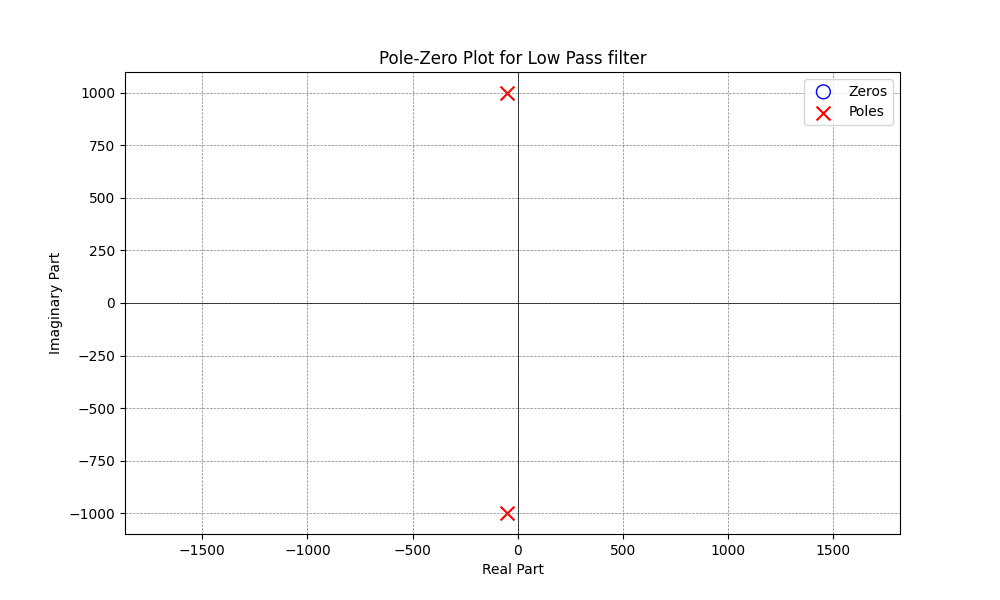
\includegraphics[keepaspectratio]{images/behaviourial/pzplot/lpf.png}}

}

\subcaption{\label{fig-bpf}Low Pass}

\end{minipage}%

\caption{\label{fig-behavioural-pole-zero}Behavioural phase and
magnitude plots}

\end{figure}%

\section{Simulation Model}\label{simulation-model}

KiCad and ngspice is used for the model simulation.

\begin{itemize}
\tightlist
\item
  We know \(\omega = \frac{1}{RC}\). We set an initial value for \(R\),
  here,\(R=1000 \Omega\). Calculating we get the \(C = 157 nF\).
\item
  We arrive at a sample circuit diagram as per Figure~\ref{fig-filter}.
\item
  Where, RA1, RB1, RC1, RC2, RC3, RD2 = R = 1000 \(\Omega\)
\item
  CA4 , CB3 = C = 157 \(nF\).
\item
  RD1 = \(Q \cdot R\),Since Q=10, RD1 = 10k \(\Omega\).
\item
  RD3 = \(R/H_0\). Since \(H_0\) = 1, RD3 = 1000 \(\Omega\).
\item
  U1A, U1B, U2A, U2B are operational amplifiers.
\item
  \(V_{in}\) is the input voltage
\item
  The outputs are take from the above mentioned op-amps. BPF from U1A,
  LPF from U1B, HPF from U2A and BSF from U2B respectively.
\end{itemize}

\begin{figure}

\centering{

\pandocbounded{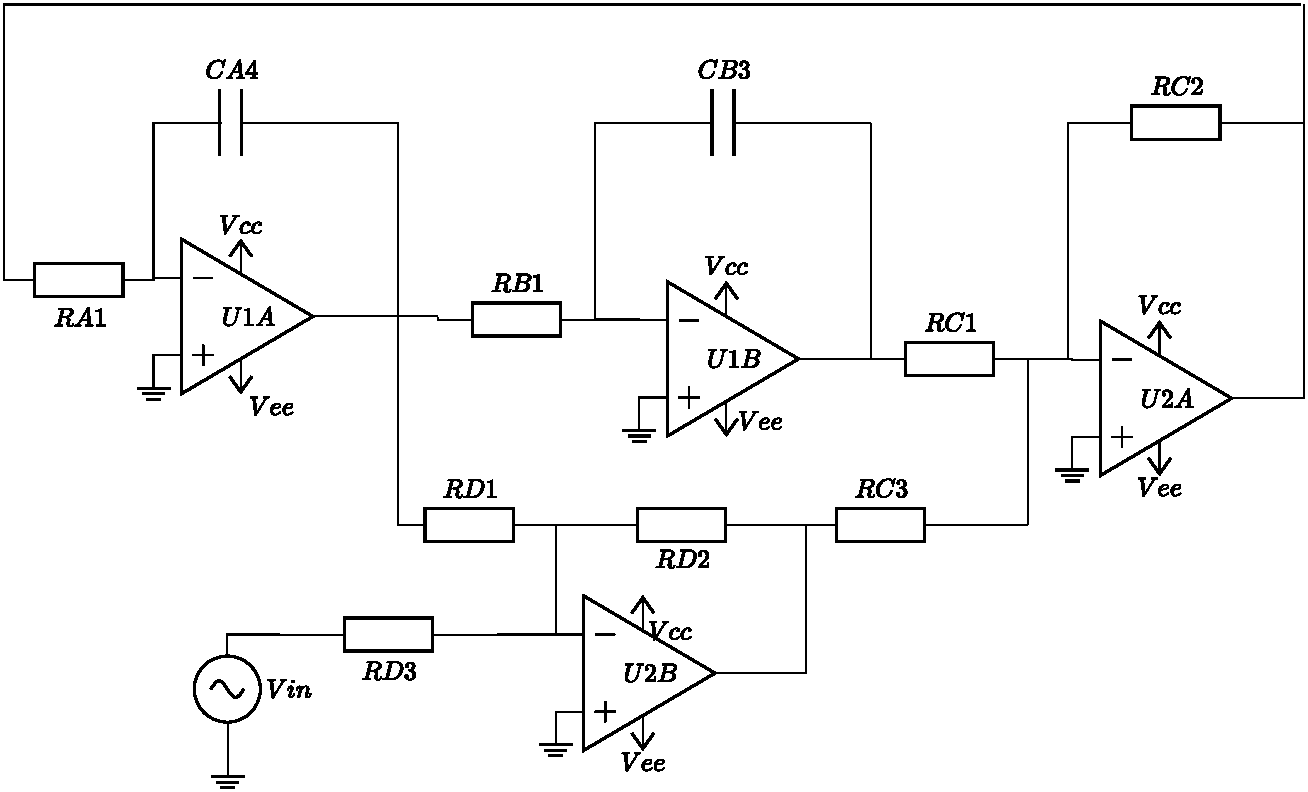
\includegraphics[keepaspectratio]{index_files/mediabag/images/FilterDiagram.pdf}}

}

\caption{\label{fig-filter}Biquad Filter Design}

\end{figure}%

The same is realised in KiCad as shown in
Figure~\ref{fig-kicadschematics}

\begin{figure}

\centering{

\pandocbounded{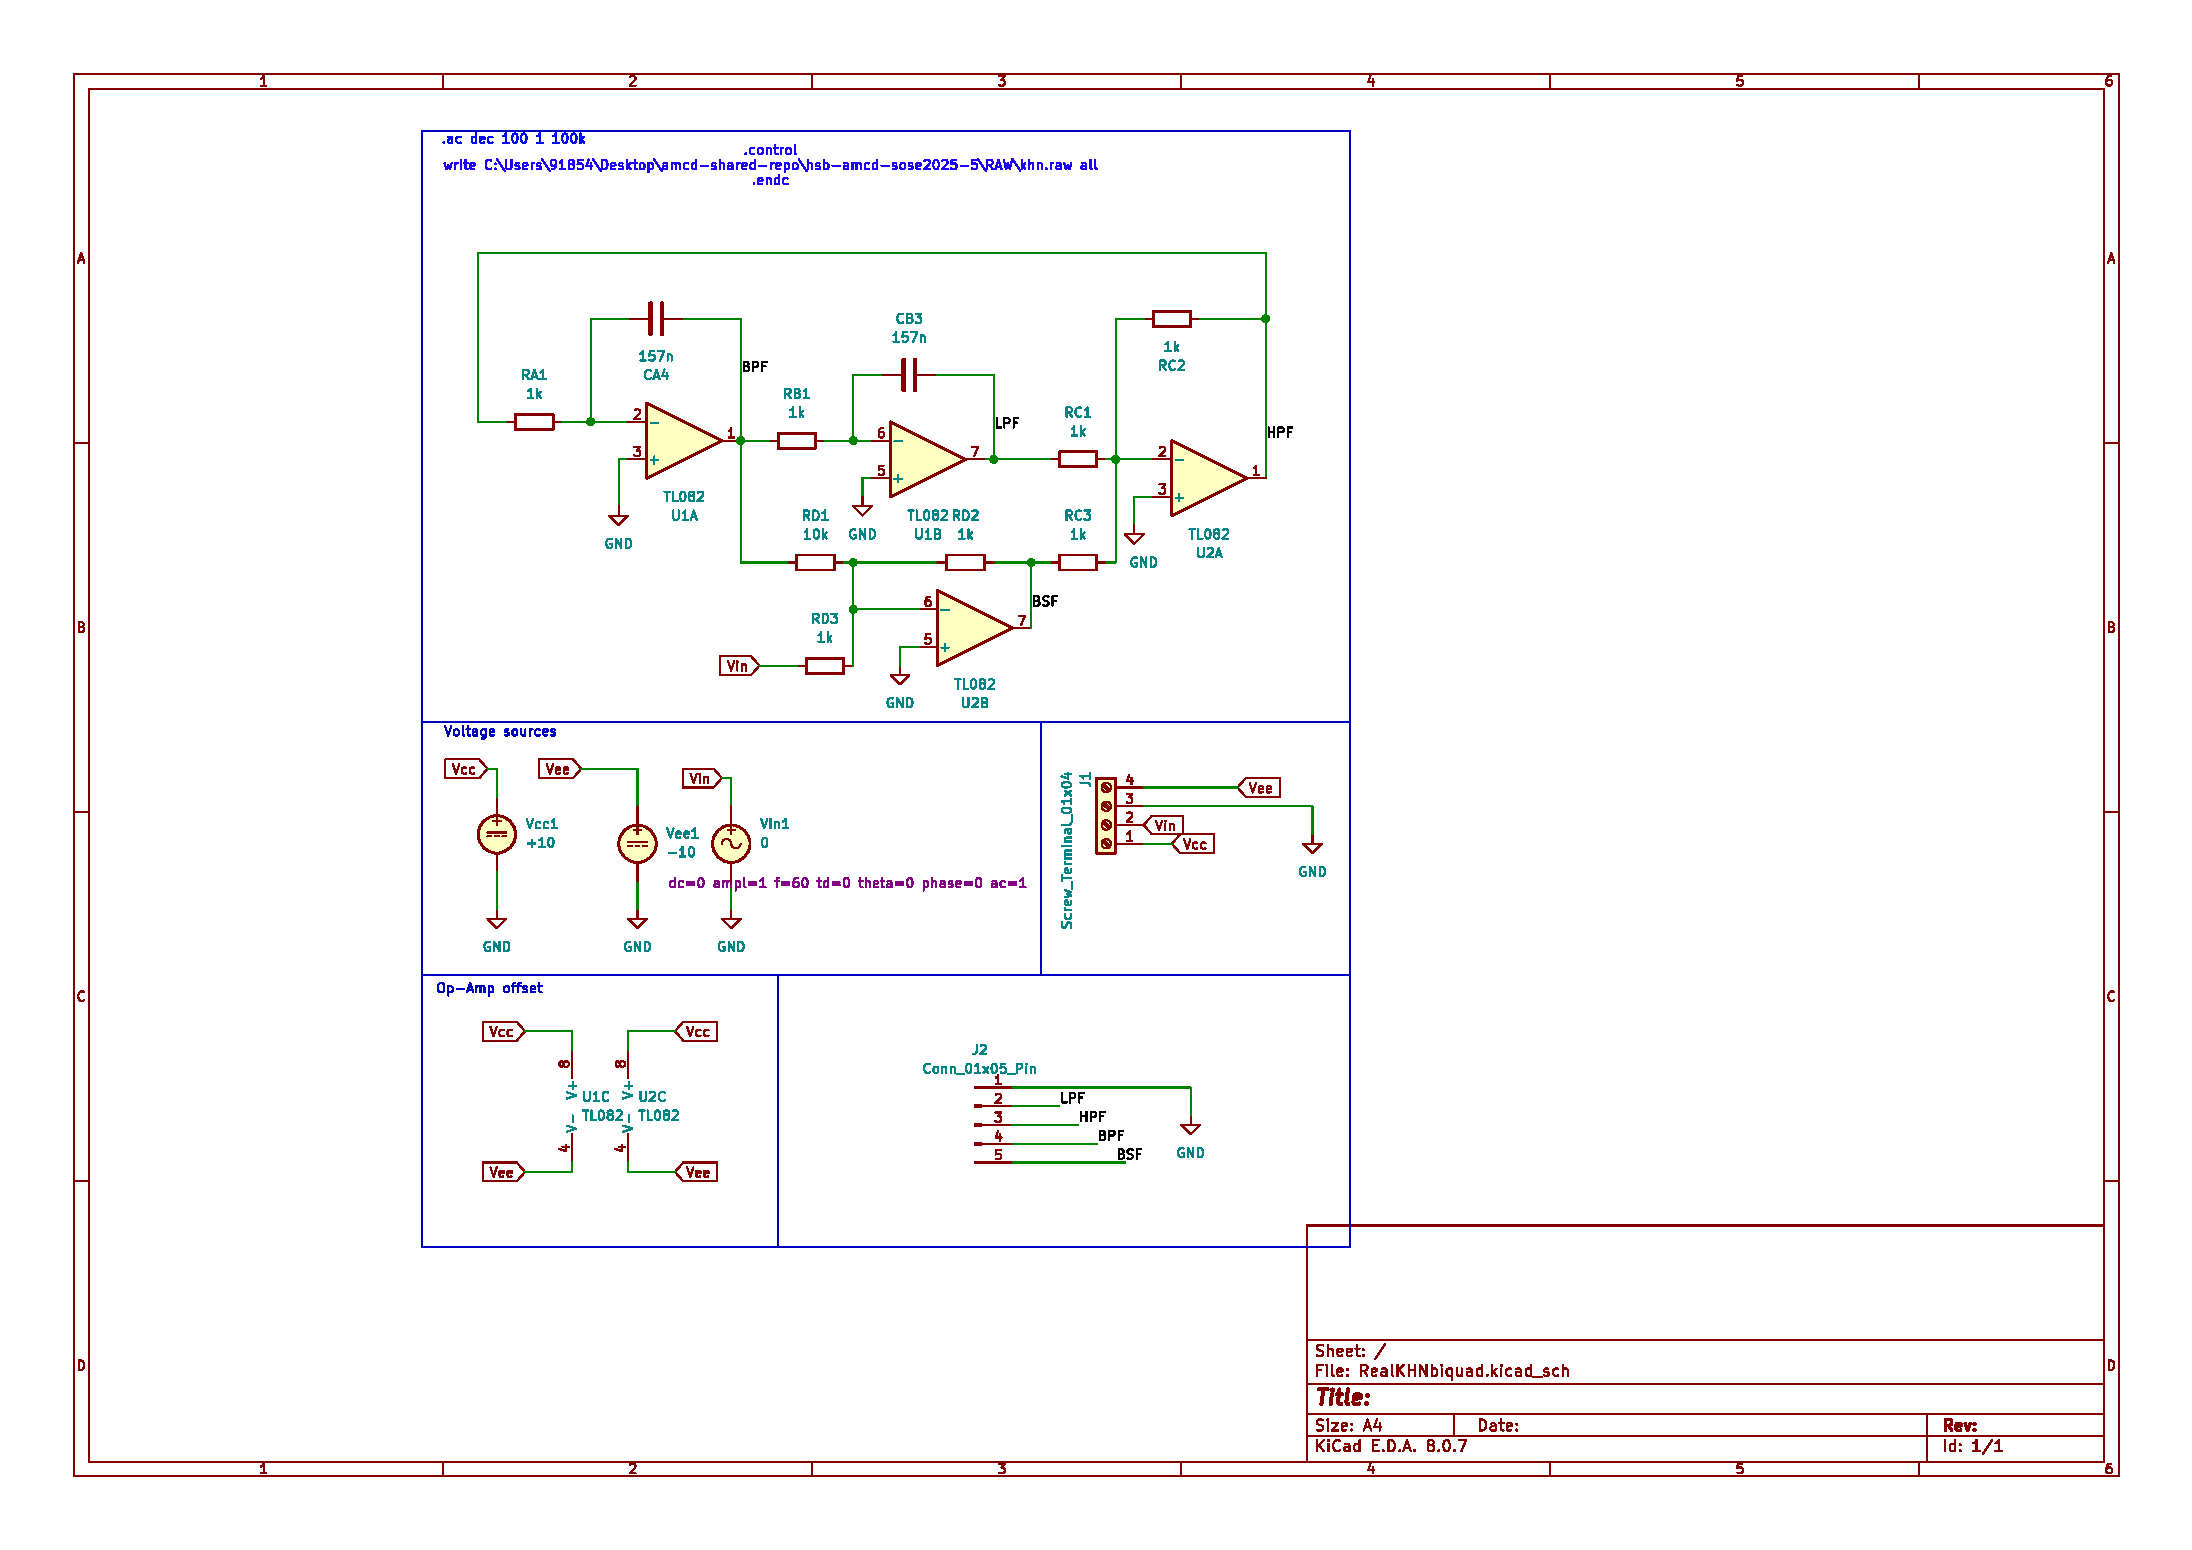
\includegraphics[keepaspectratio]{index_files/mediabag/images/breadcrumps/RealKHNbiquad.pdf}}

}

\caption{\label{fig-kicadschematics}KiCad schematics}

\end{figure}%

\subsection{\texorpdfstring{Comparison of models using
\textbf{KiCad-ngspice} and \textbf{Red Pitaya-Analog System Lab Kit
PRO}}{Comparison of models using KiCad-ngspice and Red Pitaya-Analog System Lab Kit PRO}}\label{comparison-of-models-using-kicad-ngspice-and-red-pitaya-analog-system-lab-kit-pro}

\subsubsection{ALSK Pro board circuit
connections}\label{alsk-pro-board-circuit-connections}

The circuit connections in ALSK Pro is made as
Figure~\ref{fig-alsk-connections}

\begin{figure}

\centering{

\pandocbounded{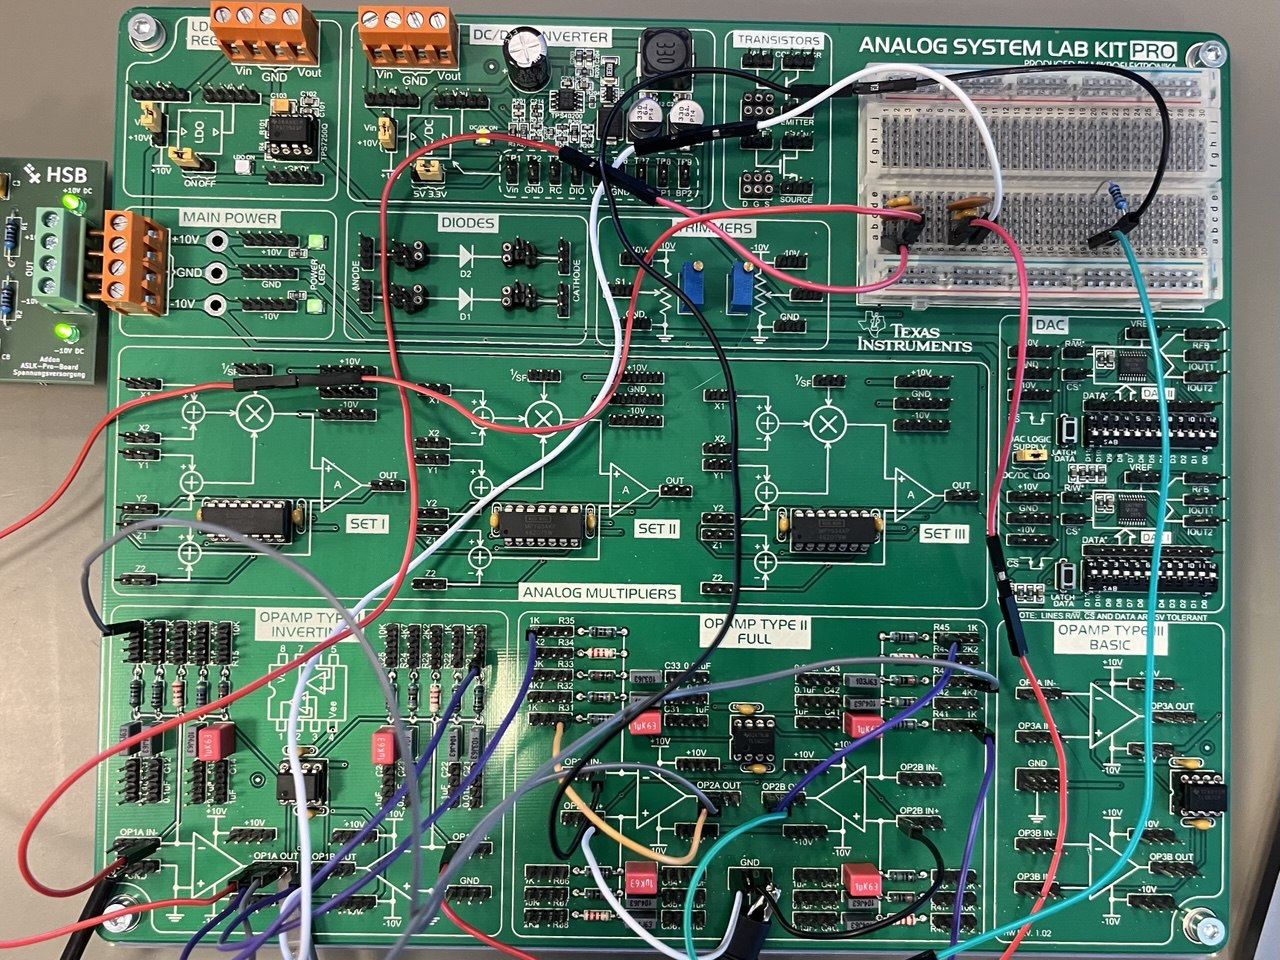
\includegraphics[keepaspectratio]{images/breadcrumps/alskdigikey.jpg}}

}

\caption{\label{fig-alsk-connections}ALSK Pro board circuit connections}

\end{figure}%

The red-pitaya module as in Figure~\ref{fig-red-pitaya-module} acts as
an oscilloscope, where the data could be taken from the server hosted by
the module.

\begin{figure}

\centering{

\pandocbounded{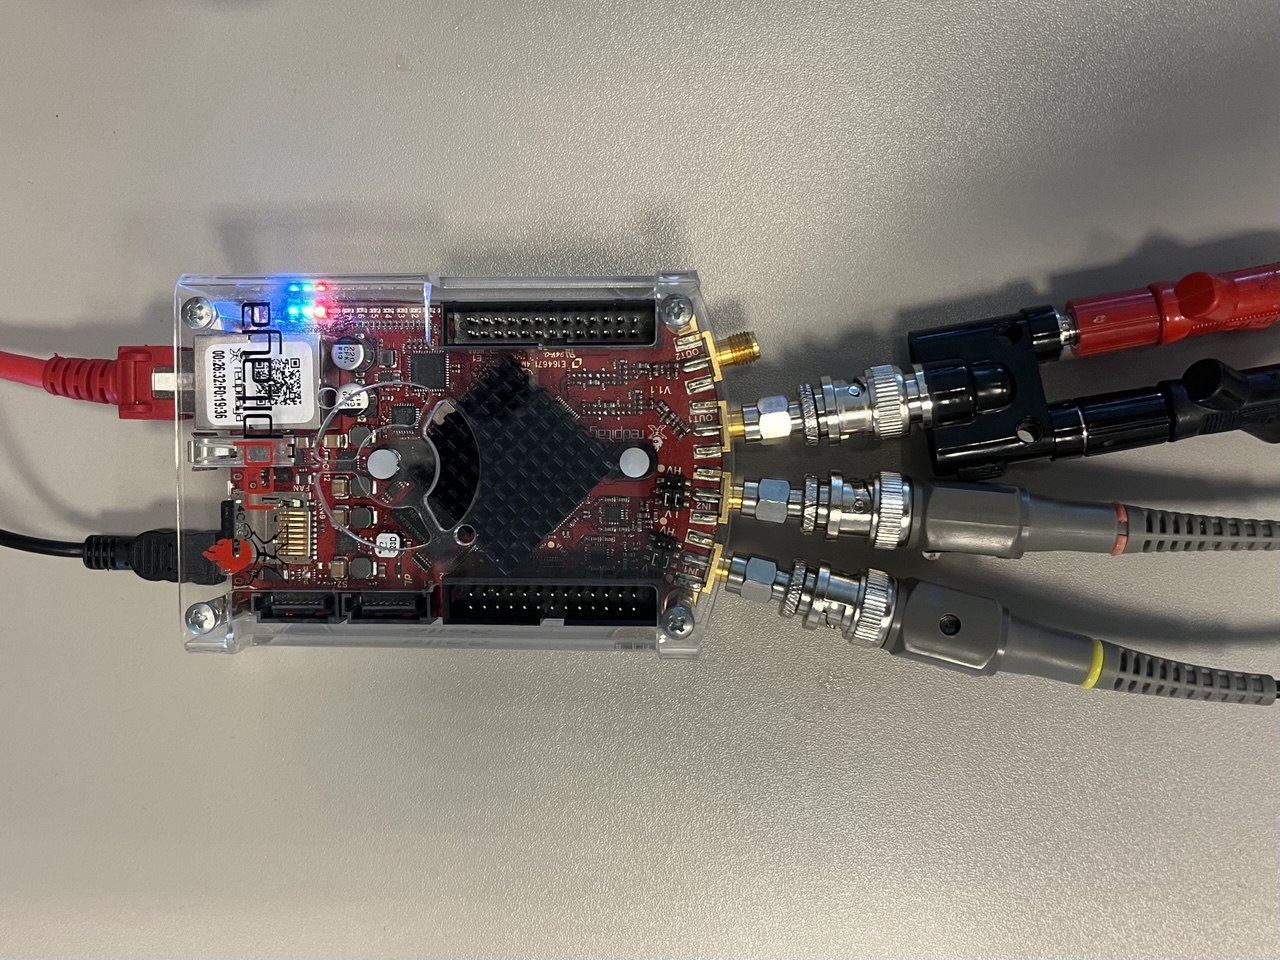
\includegraphics[keepaspectratio]{images/breadcrumps/red-pitaya.jpg}}

}

\caption{\label{fig-red-pitaya-module}Red pitaya module}

\end{figure}%

The Complete Circuit connection for the setup is shown as
Figure~\ref{fig-setup}

\begin{figure}

\centering{

\pandocbounded{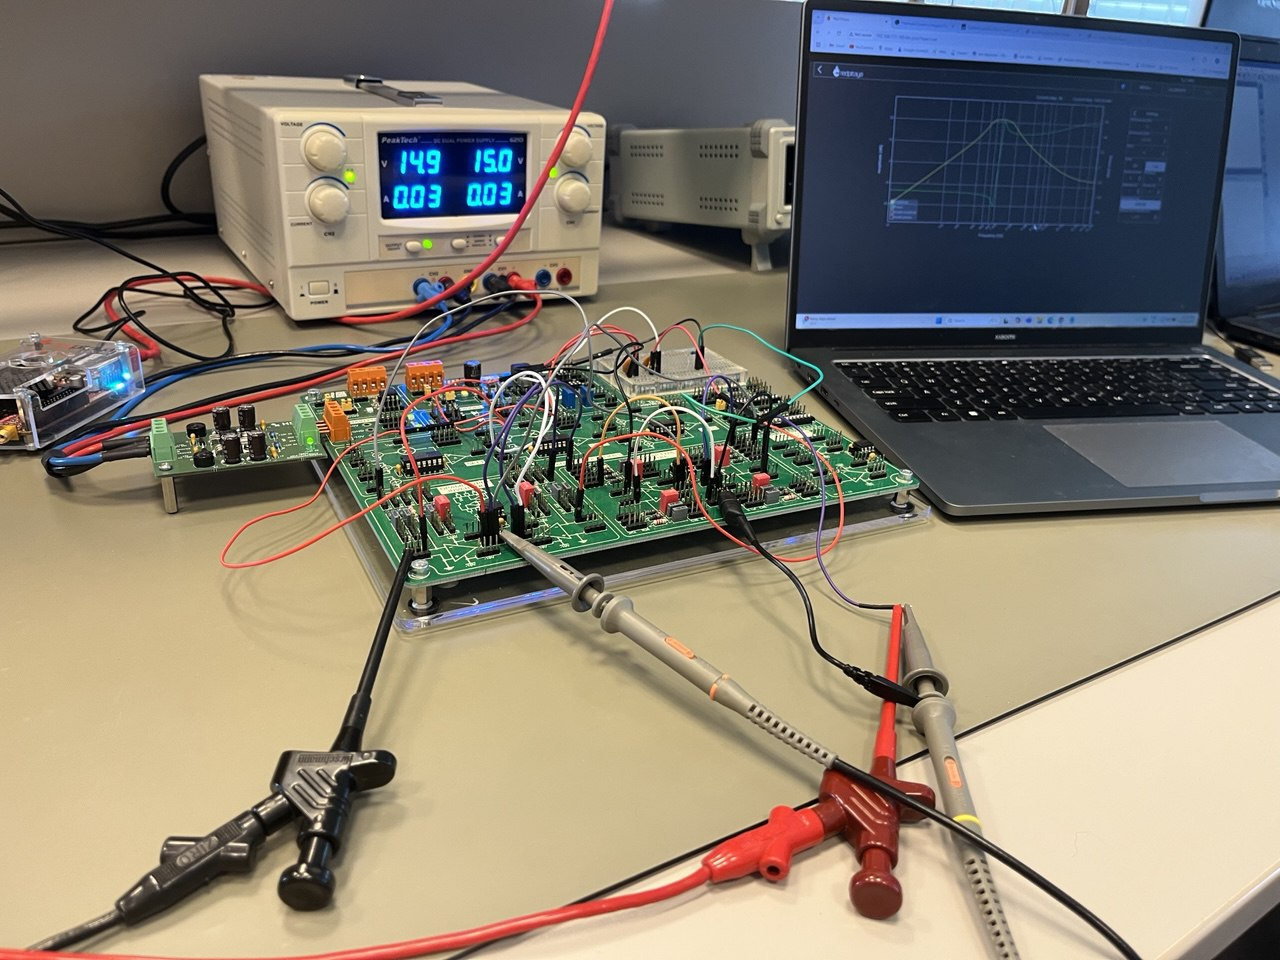
\includegraphics[keepaspectratio]{images/breadcrumps/setup.jpg}}

}

\caption{\label{fig-setup}Complete circuit connections}

\end{figure}%

\chapter{Charecteristics}\label{charecteristics}

\section{Frequency response}\label{frequency-response}

A slight variation as per Figure~\ref{fig-comparison-frequency} in
experimental model from the simulation is to be tolerated for an
acceptable inference.

\begin{figure}

\begin{minipage}{0.50\linewidth}

\centering{

\pandocbounded{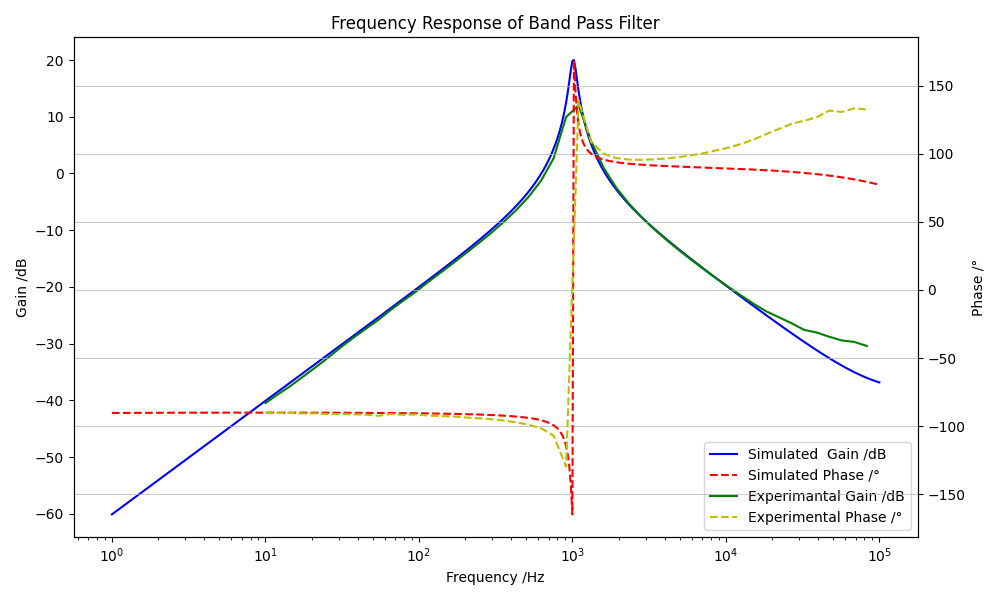
\includegraphics[keepaspectratio]{images/comparison/bode/bpf.png}}

}

\subcaption{\label{fig-bpf}Band Pass}

\end{minipage}%
%
\begin{minipage}{0.50\linewidth}

\centering{

\pandocbounded{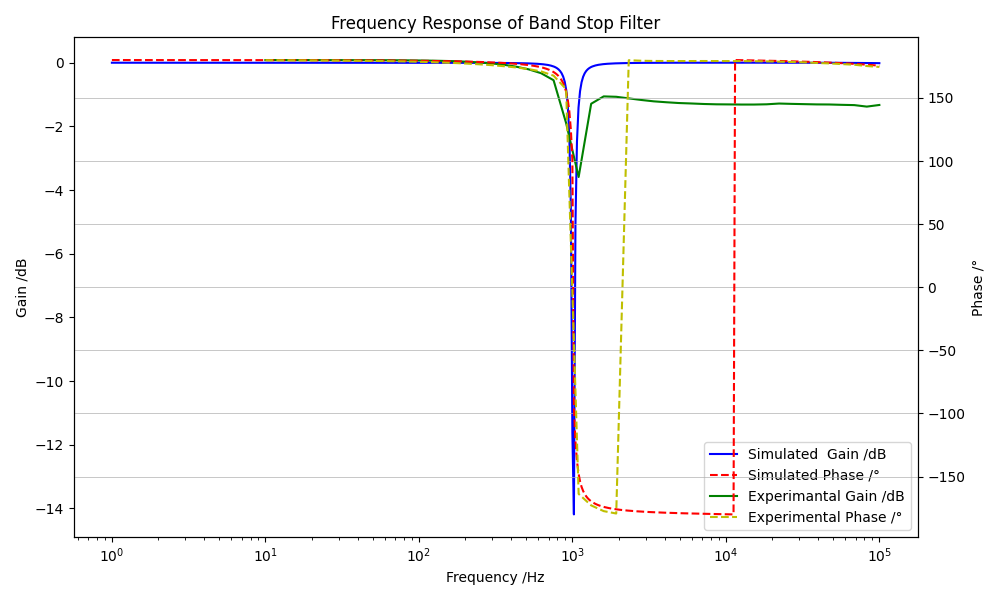
\includegraphics[keepaspectratio]{images/comparison/bode/bsf.png}}

}

\subcaption{\label{fig-bpf}Band Stop}

\end{minipage}%
\newline
\begin{minipage}{0.50\linewidth}

\centering{

\pandocbounded{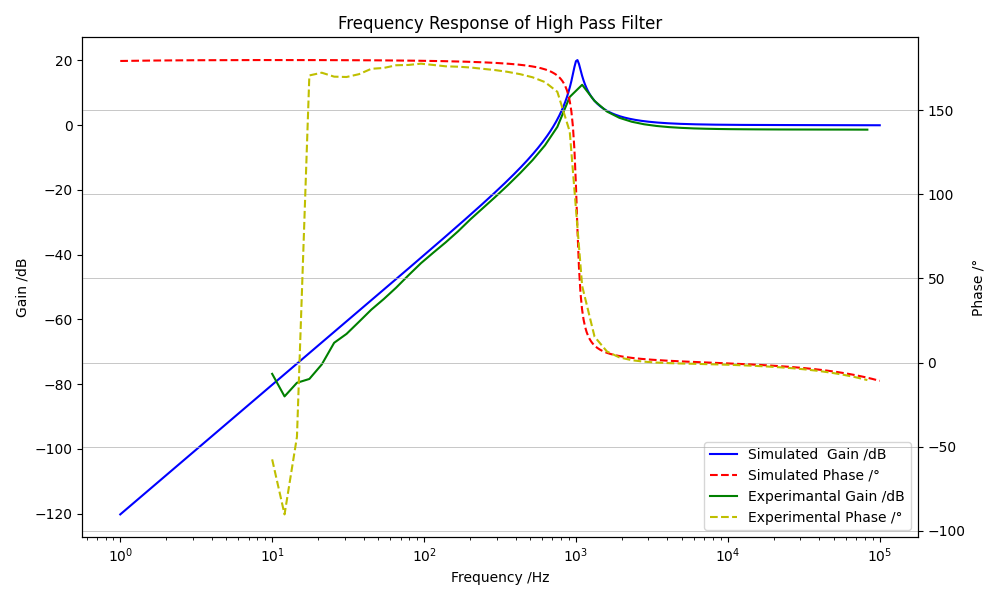
\includegraphics[keepaspectratio]{images/comparison/bode/hpf.png}}

}

\subcaption{\label{fig-bpf}High Pass}

\end{minipage}%
%
\begin{minipage}{0.50\linewidth}

\centering{

\pandocbounded{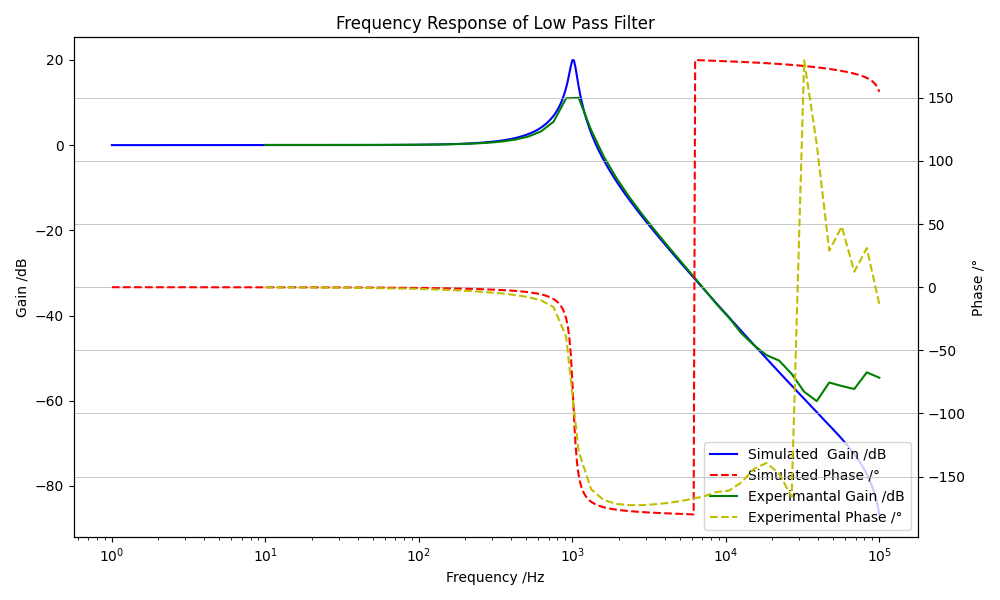
\includegraphics[keepaspectratio]{images/comparison/bode/lpf.png}}

}

\subcaption{\label{fig-bpf}Low Pass}

\end{minipage}%

\caption{\label{fig-comparison-frequency}Behavioural phase and magnitude
plots}

\end{figure}%

\section{Step response}\label{step-response}

A slight variations as per Figure~\ref{fig-comparison-transcient} in
experimental model from the simulation is to be tolerated for an
acceptable inference.

\begin{figure}

\begin{minipage}{0.50\linewidth}

\centering{

\pandocbounded{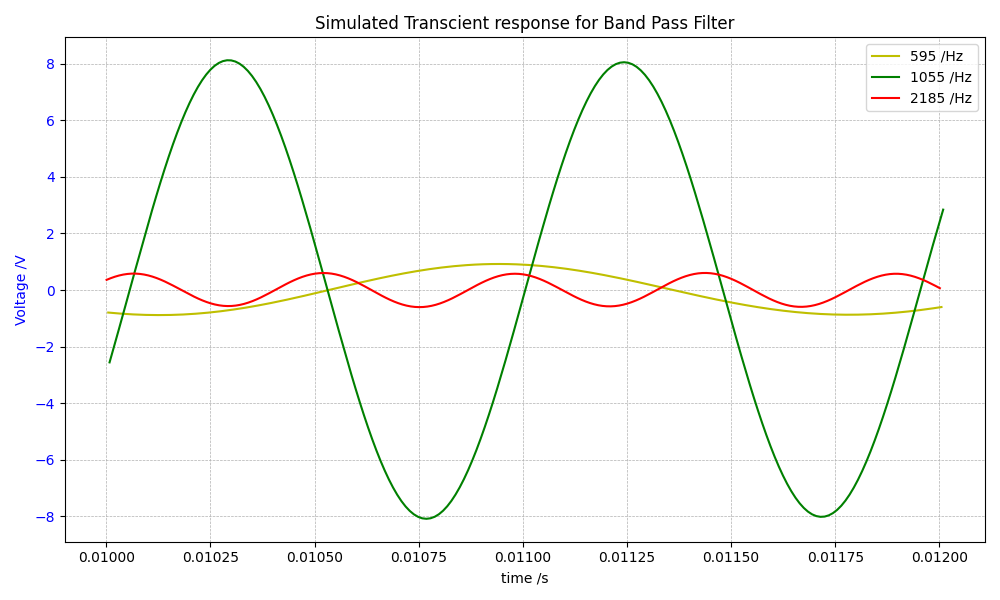
\includegraphics[keepaspectratio]{images/comparison/Transcient/Simulated/bpf.png}}

}

\subcaption{\label{fig-bpf}Simulation Band Pass}

\end{minipage}%
%
\begin{minipage}{0.50\linewidth}

\centering{

\pandocbounded{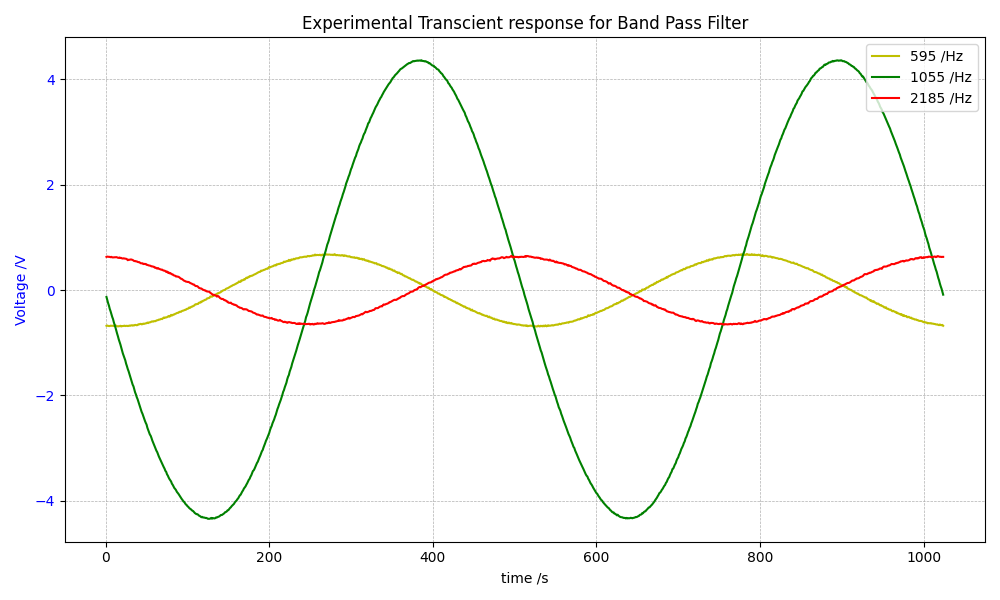
\includegraphics[keepaspectratio]{images/comparison/Transcient/experimental/bpf.png}}

}

\subcaption{\label{fig-bpf}Experimental Band Pass}

\end{minipage}%
\newline
\begin{minipage}{0.50\linewidth}

\centering{

\pandocbounded{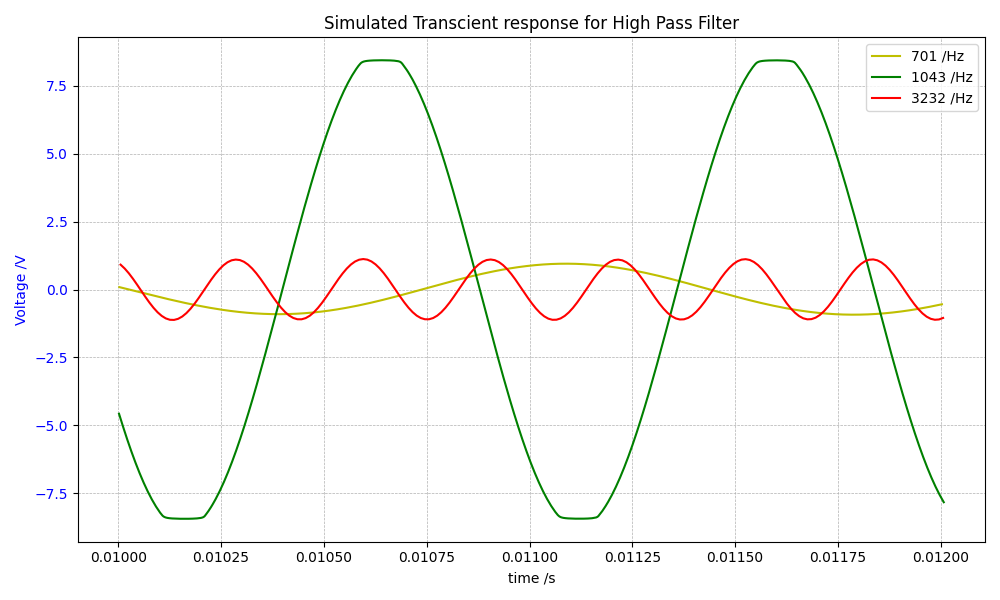
\includegraphics[keepaspectratio]{images/comparison/Transcient/Simulated/hpf.png}}

}

\subcaption{\label{fig-bpf}Simulation High Pass}

\end{minipage}%
%
\begin{minipage}{0.50\linewidth}

\centering{

\pandocbounded{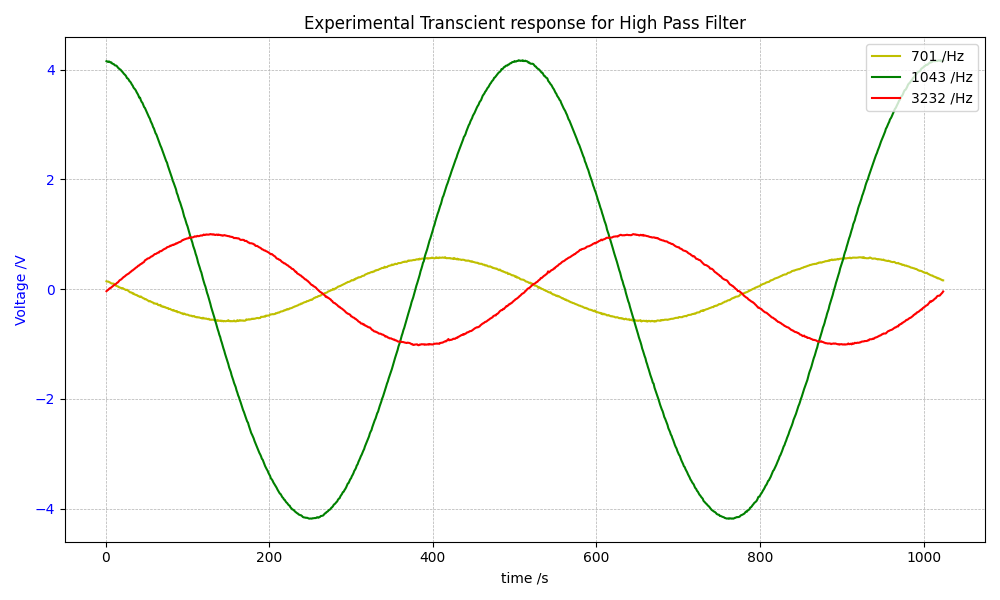
\includegraphics[keepaspectratio]{images/comparison/Transcient/experimental/hpf.png}}

}

\subcaption{\label{fig-bpf}Experimental High Pass}

\end{minipage}%
\newline
\begin{minipage}{0.50\linewidth}

\centering{

\pandocbounded{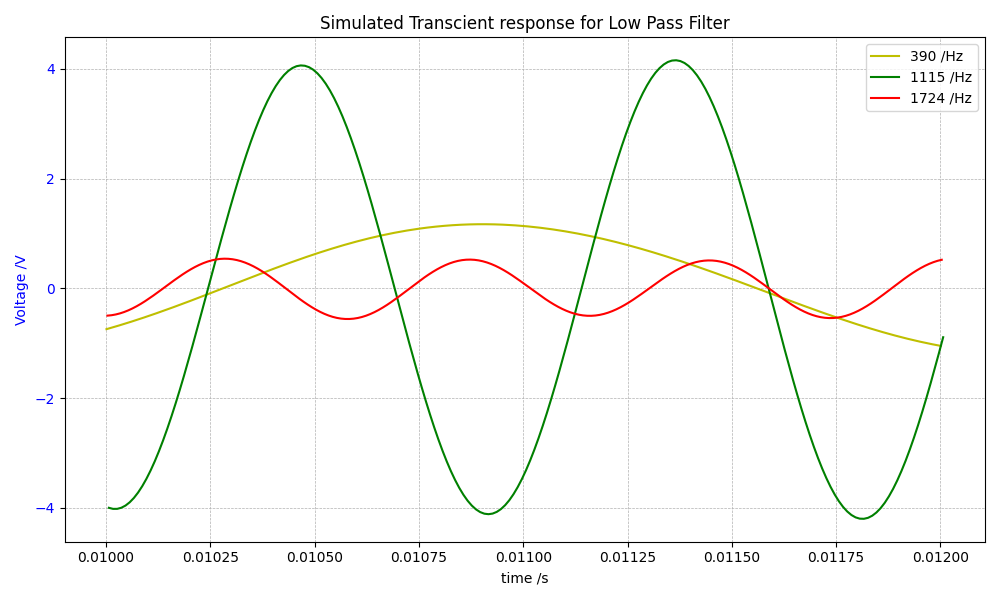
\includegraphics[keepaspectratio]{images/comparison/Transcient/Simulated/lpf.png}}

}

\subcaption{\label{fig-bpf}Simulation Low Pass}

\end{minipage}%
%
\begin{minipage}{0.50\linewidth}

\centering{

\pandocbounded{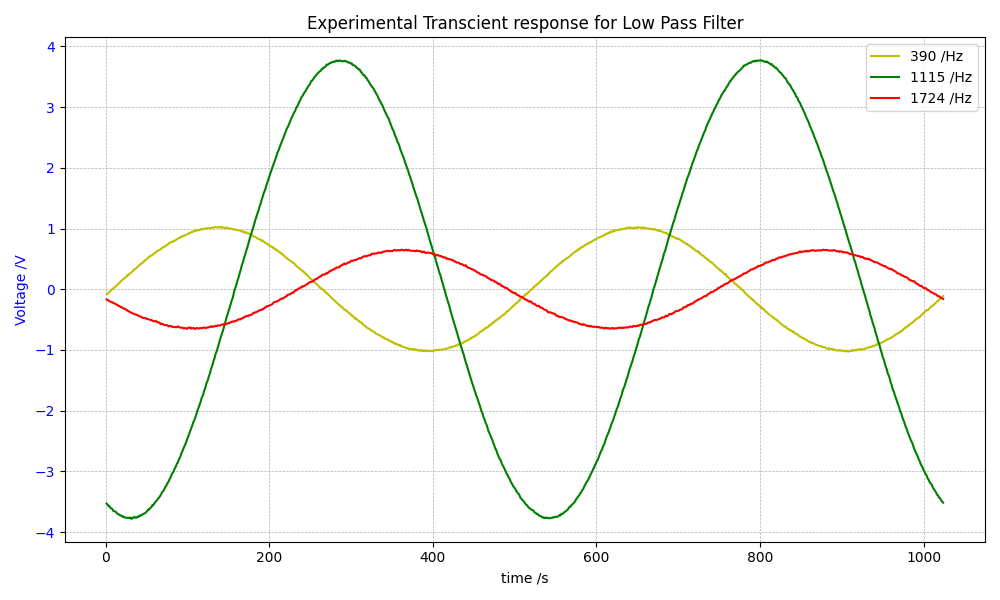
\includegraphics[keepaspectratio]{images/comparison/Transcient/experimental/lpf.png}}

}

\subcaption{\label{fig-bpf}Experimental Low Pass}

\end{minipage}%
\newline
\begin{minipage}{0.50\linewidth}

\centering{

\pandocbounded{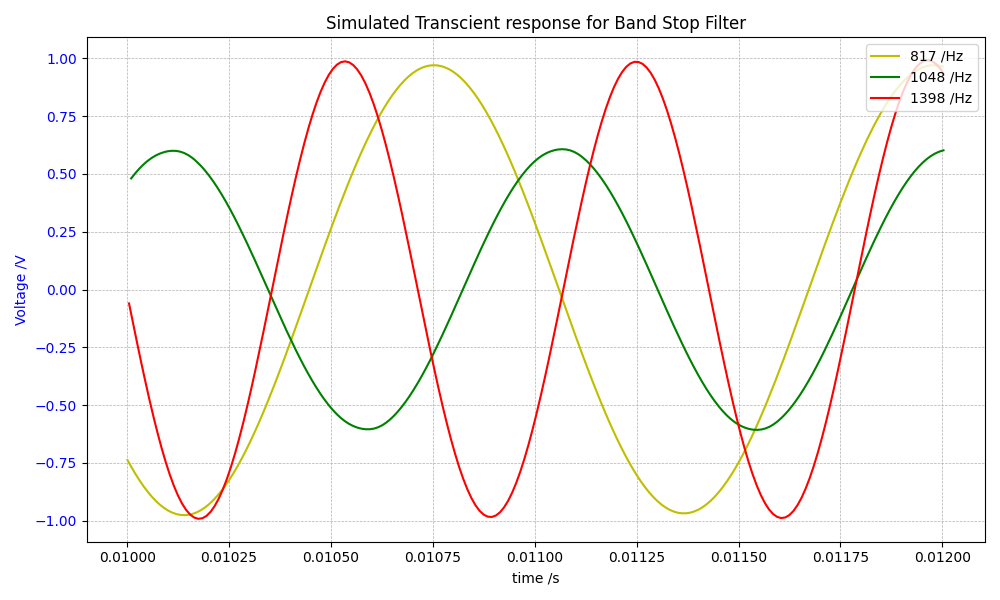
\includegraphics[keepaspectratio]{images/comparison/Transcient/Simulated/bsf.png}}

}

\subcaption{\label{fig-bpf}Simulation Band Stop}

\end{minipage}%
%
\begin{minipage}{0.50\linewidth}

\centering{

\pandocbounded{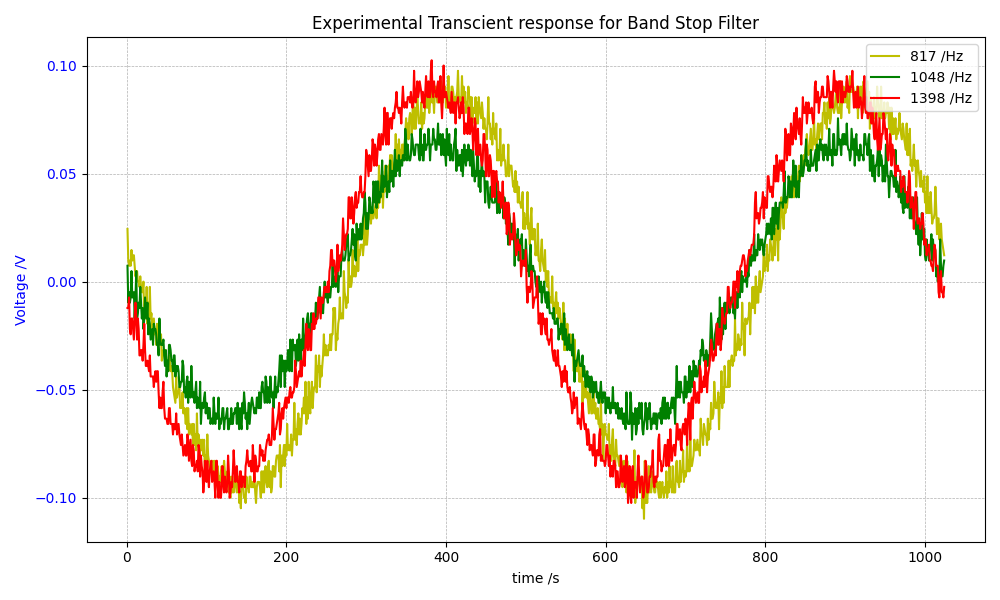
\includegraphics[keepaspectratio]{images/comparison/Transcient/experimental/bsf.png}}

}

\subcaption{\label{fig-bpf}Experimental Band Stop}

\end{minipage}%

\caption{\label{fig-comparison-transcient}Comparison of step response}

\end{figure}%

\chapter{PCB Design using KiCAD}\label{pcb-design-using-kicad}

From the above Figure~\ref{fig-kicadschematics} , we get can generate a
PCB Layout. Care is taken to avoid signal interference. The track width
is chosen to be 0.025 inches or 0.635 mm. The number of via's and 90
degree tracks are reduced and avoided.

\section{PCB 2D Layout}\label{pcb-2d-layout}

Most of the SMD(Surface Mount Devices) are chosen with 0805 variants.
For the op-amp, the spice model, 3D model and footprint is downloaded
from official
\href{https://www.ti.com/product/TL082\#design-tools-simulation}{ti
website}. The DRC check and zone filling of voltages in PCB is also
done.

\begin{figure}

\begin{minipage}{0.50\linewidth}

\pandocbounded{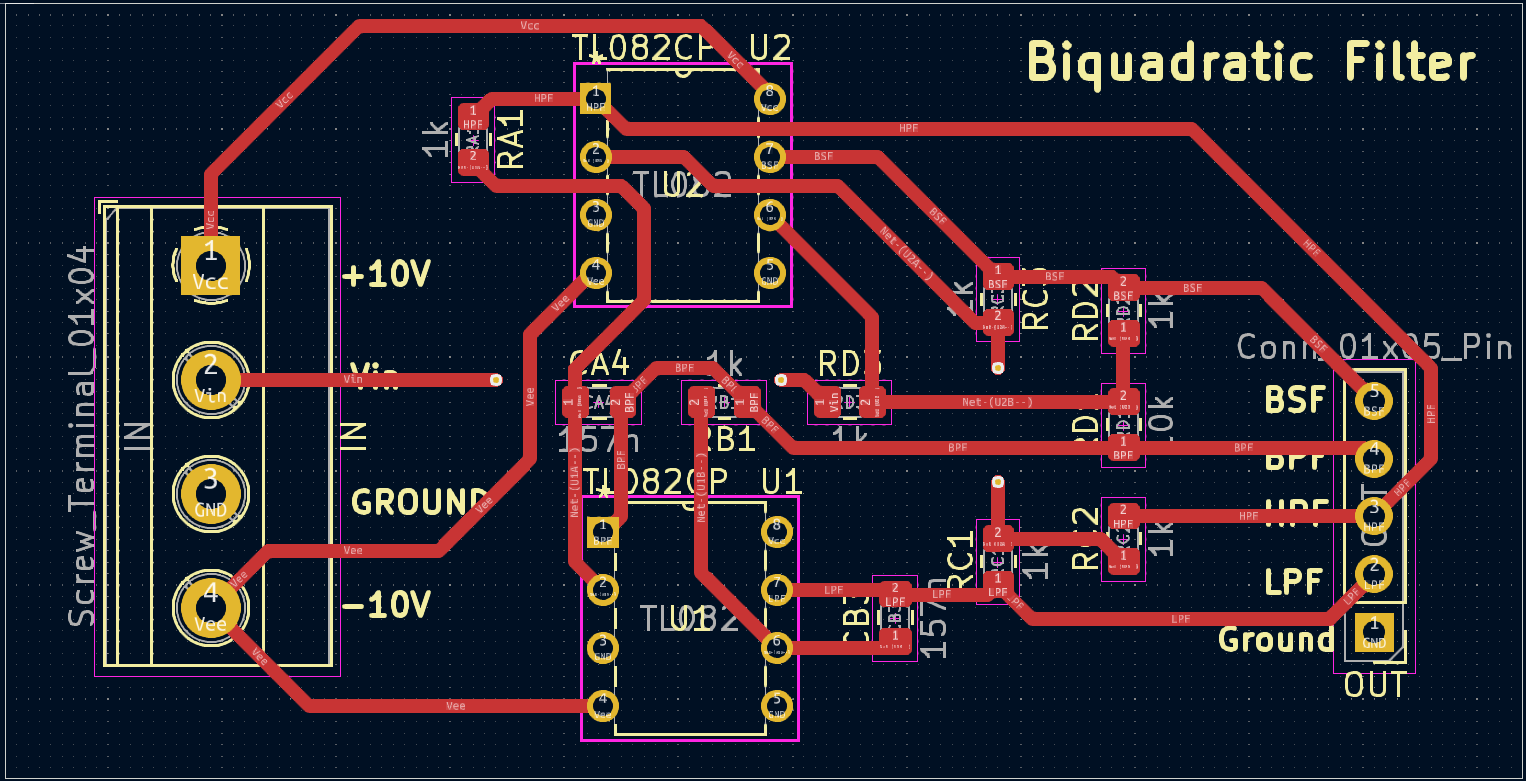
\includegraphics[keepaspectratio]{images/PCB/fpcb2d.png}}

\subcaption{\label{}PCB Front}
\end{minipage}%
%
\begin{minipage}{0.50\linewidth}

\pandocbounded{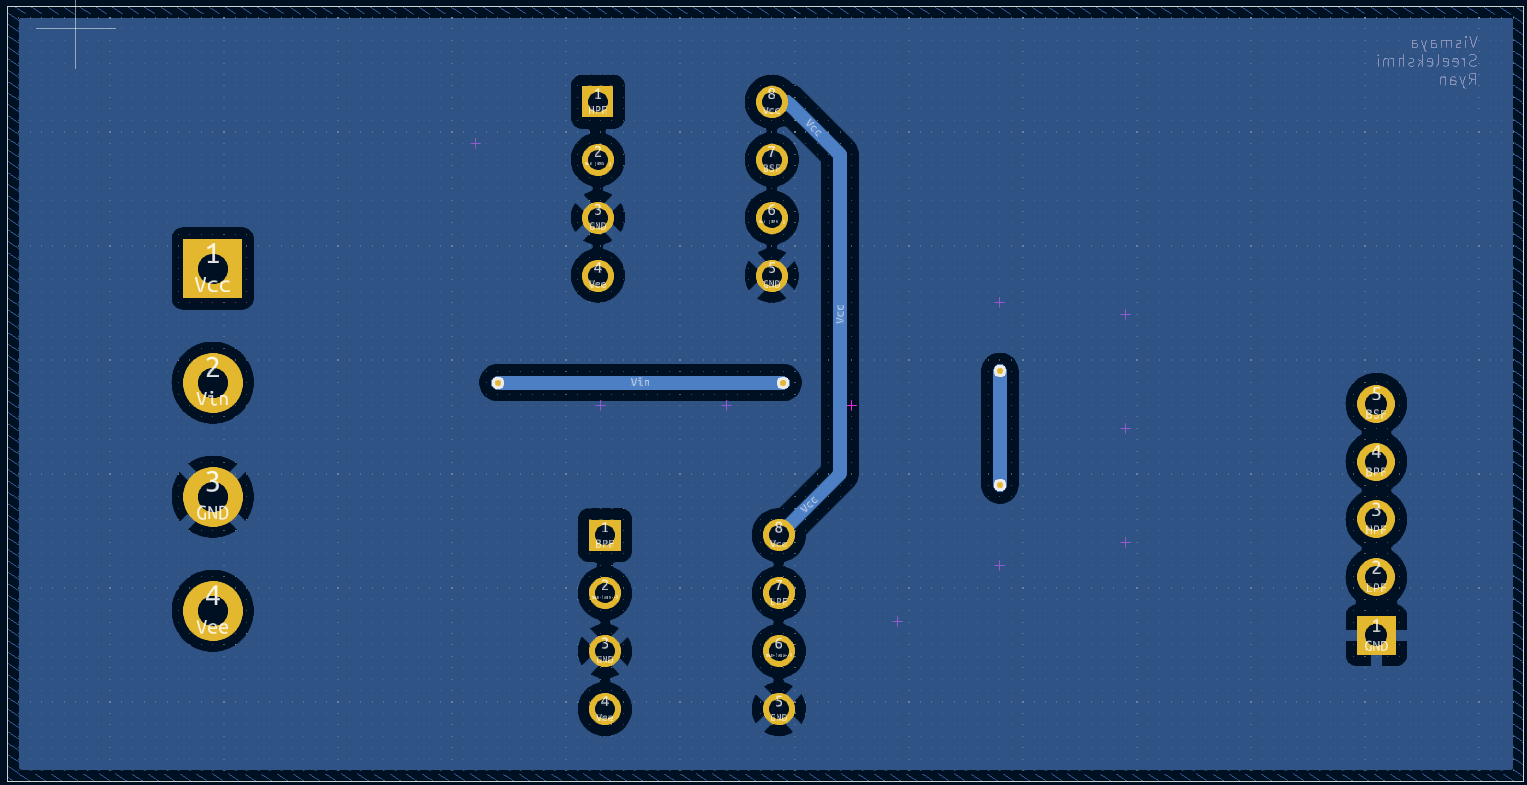
\includegraphics[keepaspectratio]{images/PCB/bpcb2d.png}}

\subcaption{\label{}PCB Back}
\end{minipage}%

\caption{\label{fig-pcb-2d}PCB 2D Layout}

\end{figure}%

\section{PCB 3D Rendered View}\label{pcb-3d-rendered-view}

The 3D model of all devices including the op-amp is loaded from the
official websites and hence rendered. The final view is cross verified.

\begin{figure}

\begin{minipage}{0.50\linewidth}

\pandocbounded{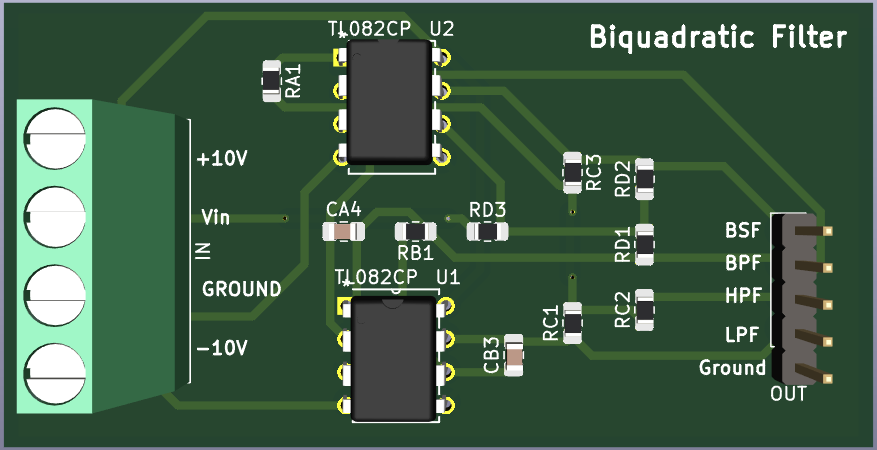
\includegraphics[keepaspectratio]{images/PCB/fpcb.png}}

\subcaption{\label{}PCB Front}
\end{minipage}%
%
\begin{minipage}{0.50\linewidth}

\pandocbounded{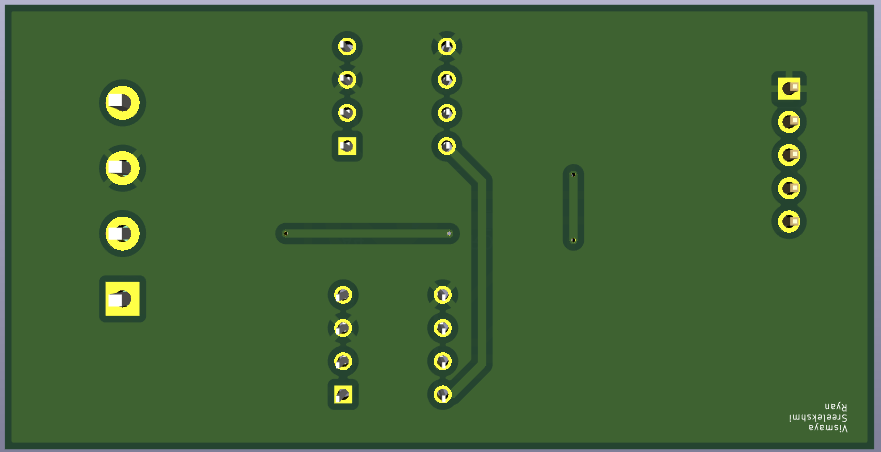
\includegraphics[keepaspectratio]{images/PCB/bpcb.png}}

\subcaption{\label{}PCB Back}
\end{minipage}%

\caption{\label{fig-pcb-3d}PCB 3D rendered view}

\end{figure}%

\section{PCB Board images}\label{pcb-board-images}

\begin{figure}[H]

{\centering 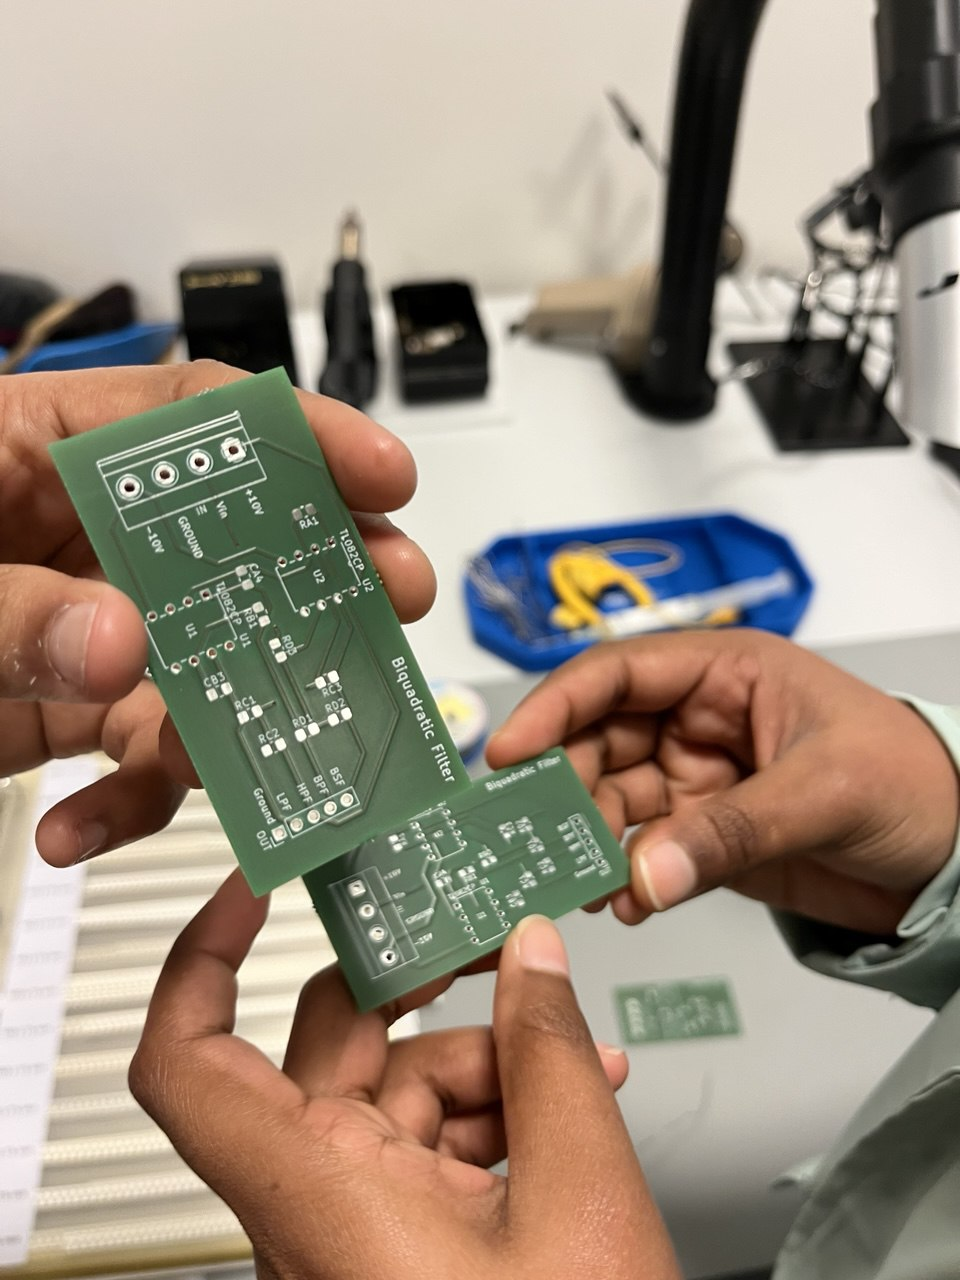
\includegraphics[width=\linewidth,height=5.20833in,keepaspectratio]{images/breadcrumps/boardBeforeSoldering.jpg}

}

\caption{PCB Board before soldering}

\end{figure}%

\begin{figure}[H]

{\centering 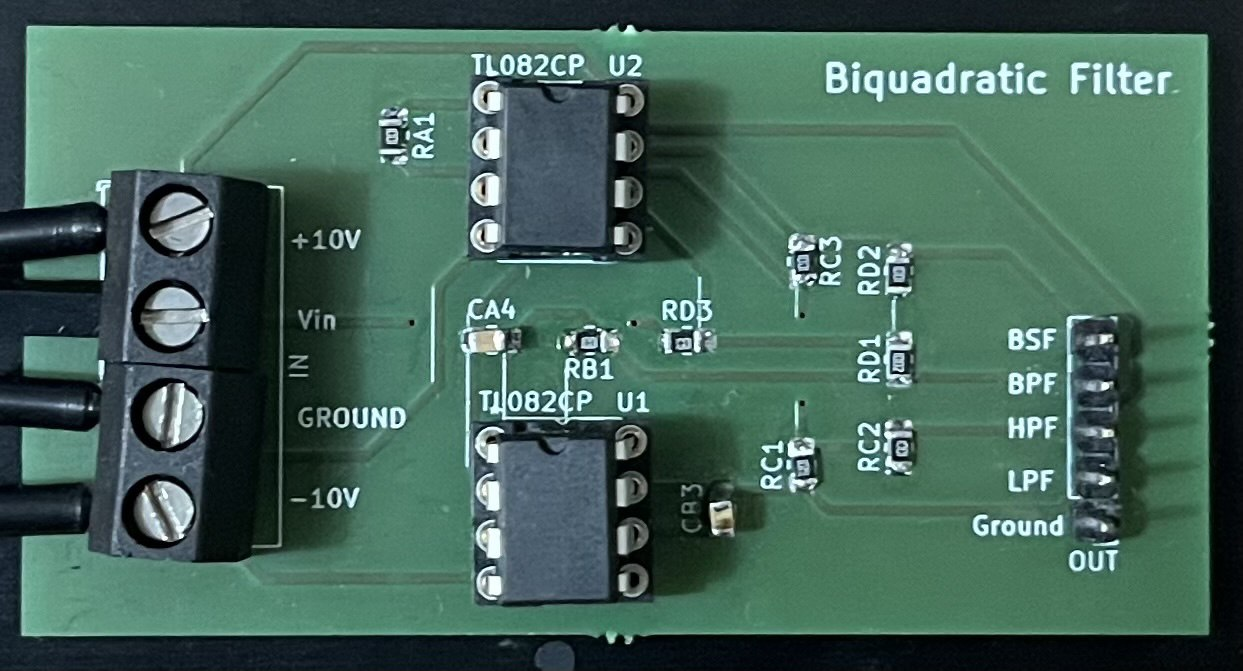
\includegraphics[width=\linewidth,height=4.16667in,keepaspectratio]{images/breadcrumps/finalBoard.jpg}

}

\caption{PCB Board after soldering}

\end{figure}%

\chapter{PCB Charecteristics}\label{pcb-charecteristics}

\section{Frequency Analysis}\label{frequency-analysis}

\begin{figure}

\begin{minipage}{0.50\linewidth}

\centering{

\pandocbounded{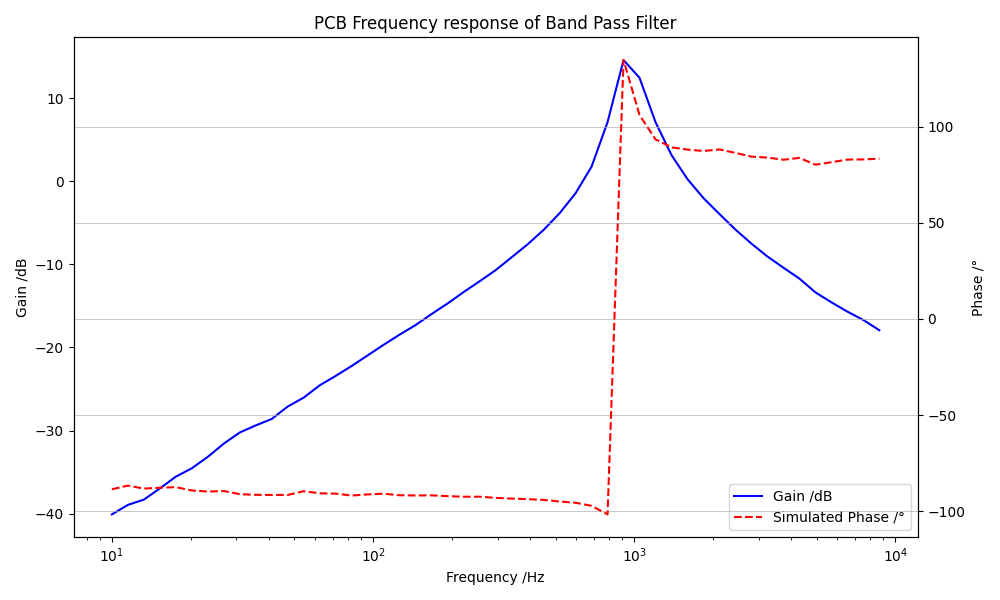
\includegraphics[keepaspectratio]{images/PCB/bode/bpf.png}}

}

\subcaption{\label{fig-bpf}Band Pass}

\end{minipage}%
%
\begin{minipage}{0.50\linewidth}

\centering{

\pandocbounded{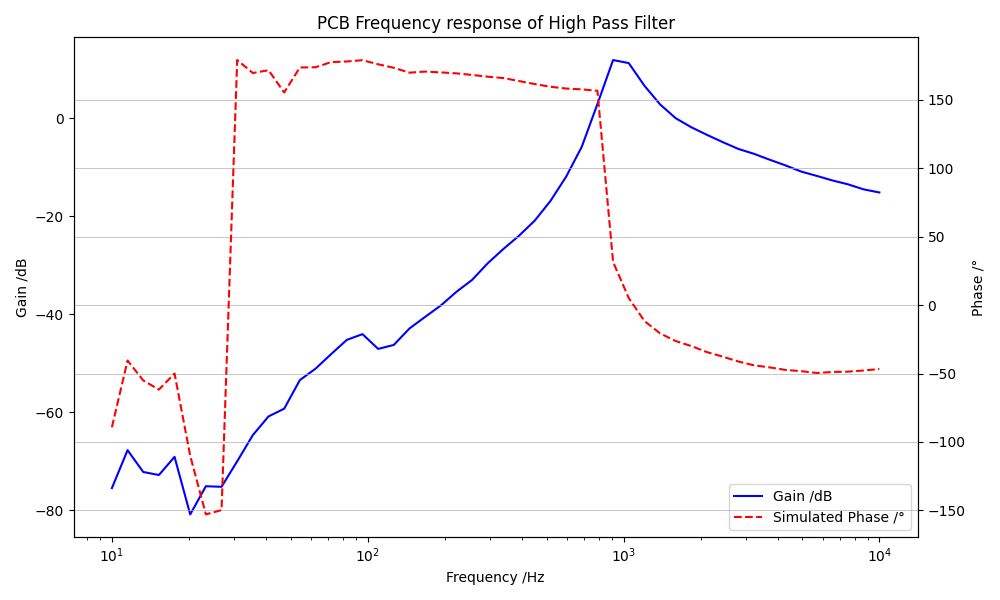
\includegraphics[keepaspectratio]{images/PCB/bode/hpf.png}}

}

\subcaption{\label{fig-bpf}High Pass}

\end{minipage}%
\newline
\begin{minipage}{0.50\linewidth}

\centering{

\pandocbounded{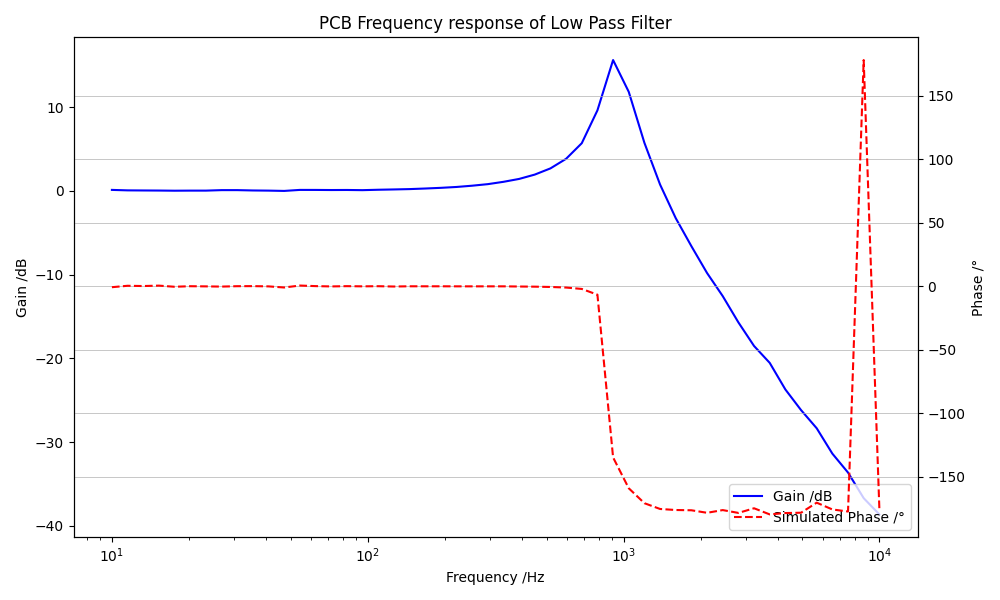
\includegraphics[keepaspectratio]{images/PCB/bode/lpf.png}}

}

\subcaption{\label{fig-bpf}Low Pass}

\end{minipage}%

\caption{\label{fig-pcb-frequency}Frequency Analysis}

\end{figure}%

\section{Transcient Analysis}\label{transcient-analysis}

\begin{figure}

\begin{minipage}{0.50\linewidth}

\centering{

\pandocbounded{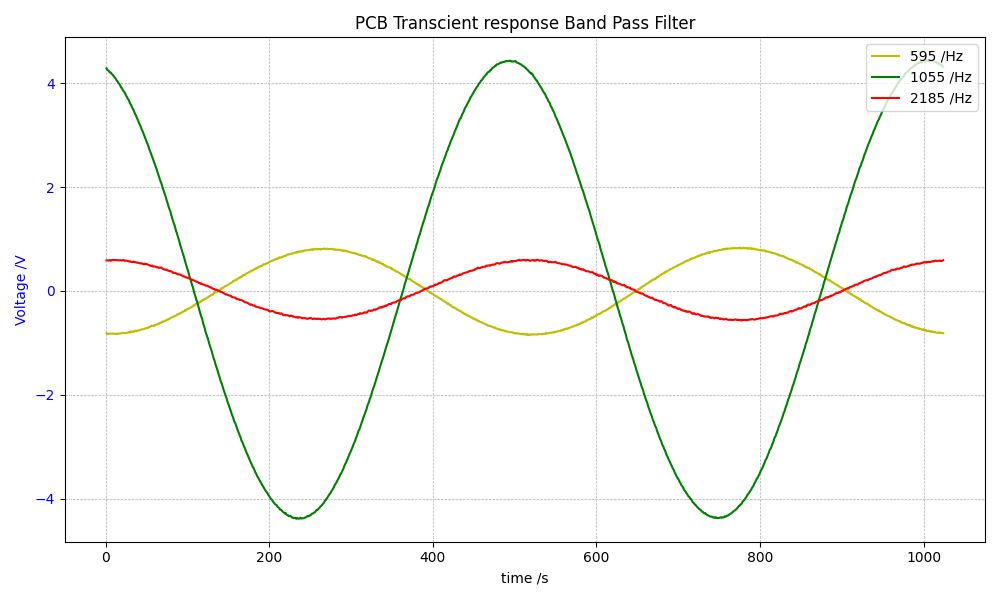
\includegraphics[keepaspectratio]{images/PCB/Transcient/bpf.png}}

}

\subcaption{\label{fig-bpf}Band Pass}

\end{minipage}%
%
\begin{minipage}{0.50\linewidth}

\centering{

\pandocbounded{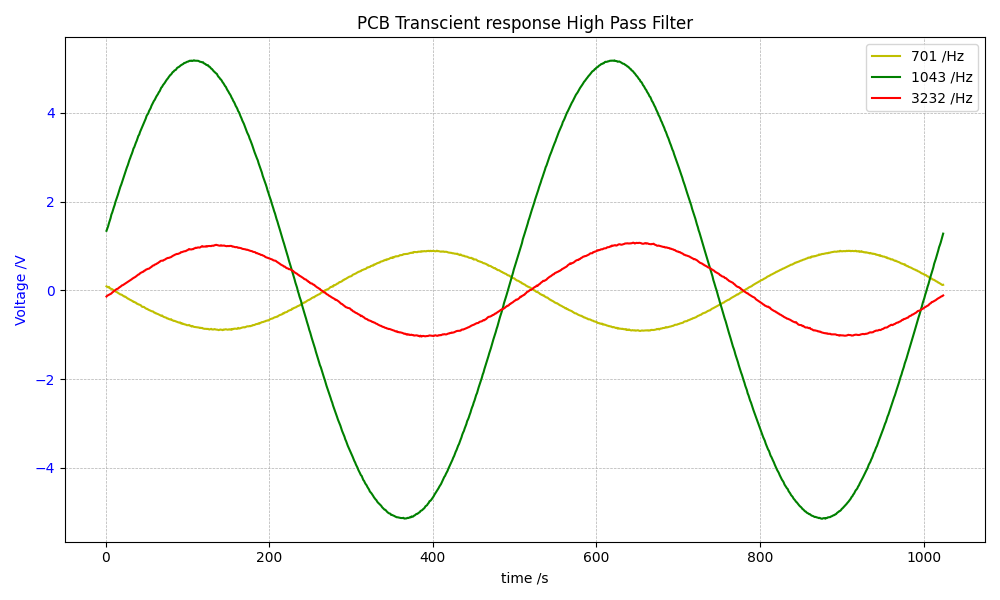
\includegraphics[keepaspectratio]{images/PCB/Transcient/hpf.png}}

}

\subcaption{\label{fig-bpf}High Pass}

\end{minipage}%
\newline
\begin{minipage}{0.50\linewidth}

\centering{

\pandocbounded{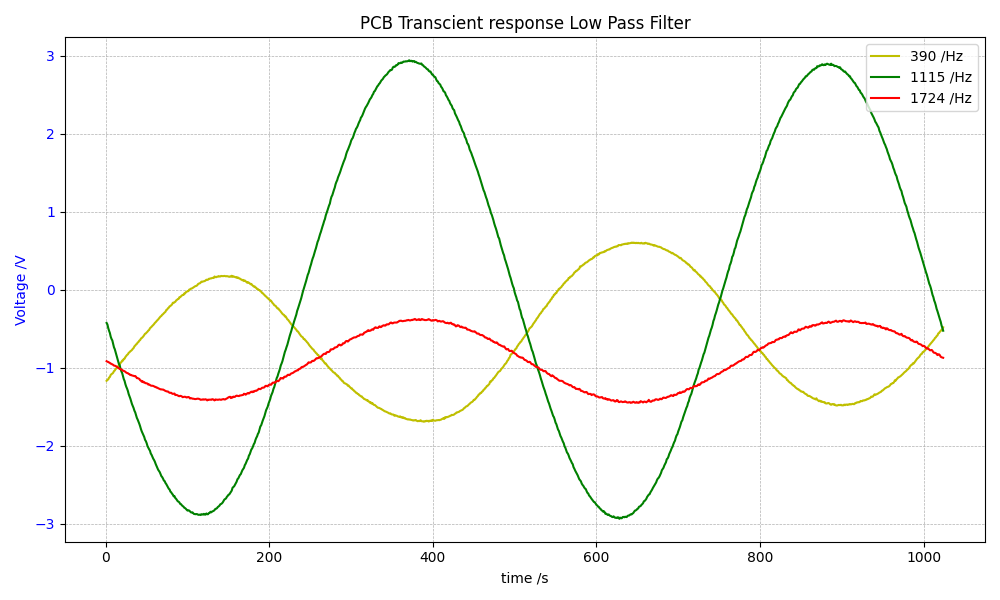
\includegraphics[keepaspectratio]{images/PCB/Transcient/lpf.png}}

}

\subcaption{\label{fig-bpf}Low Pass}

\end{minipage}%

\caption{\label{fig-pcb-transcient}Transcient Analysis}

\end{figure}%

\chapter{Conclusion}\label{conclusion}

The project successfully demonstrated the complete design and
implementation of a universal biquad filter across behavioral modeling,
simulation, ASLK PRO, and PCB levels. High-pass, low-pass, and band-pass
filter configurations were realized with results that closely aligned
with expected theoretical characteristics. These outcomes validate the
robustness of the design methodology and the effectiveness of the
development workflow.

While the band-stop filter (BSF) at the PCB level did not yield optimal
performance, likely due to signal noise or interference in the layout,
this isolated issue does not overshadow the overall success of the
project. On the contrary, it highlights valuable areas for further
refinement in PCB design and noise mitigation. The experience reinforces
the importance of layout considerations and serves as a stepping stone
for future enhancements.

Overall, the project showcases a comprehensive and reproducible analog
design flow---from concept to hardware---using modern, open-source tools
and platforms.

\chapter*{References}\label{references}
\addcontentsline{toc}{chapter}{References}

\phantomsection\label{refs}
\begin{CSLReferences}{1}{0}
\bibitem[\citeproctext]{ref-baker2010}
Baker, R. Jacob. 2010. \emph{{CMOS}: Circuit Design, Layout, and
Simulation}. 3rd ed. Wiley-IEEE Press.
\url{https://doi.org/10.1002/9780470891179}.

\bibitem[\citeproctext]{ref-stanfordEE315}
{``EE315 Course.''} 2025. Stanford University;
\url{https://explorecourses.stanford.edu/search?view=catalog&filter-coursestatus-Active=on&page=0&catalog=&academicYear=&q=ee315}.

\end{CSLReferences}




\end{document}
